\documentclass{wissdoc}

% Autor: Roland Bless 1996-2009, bless <at> kit.edu
% ----------------------------------------------------------------
% Diplomarbeit - Hauptdokument
% ----------------------------------------------------------------
%%
%% $Id: diplarb.tex 53 2009-12-10 12:23:37Z bless $
%%
% wissdoc Optionen: draft, relaxed, pdf --> siehe wissdoc.cls
% ------------------------------------------------------------------
% Weitere packages: (Dokumentation dazu durch "latex <package>.dtx")
%\usepackage{bibgerm}
%\usepackage[backend=biber]{biblatex}
\usepackage{csquotes}
\usepackage{tabularx}
\usepackage{booktabs}
\usepackage{multirow}
%\usepackage{tocbibind}
\usepackage{siunitx}
\usepackage{xcolor}
\usepackage{textcomp}
\usepackage{listings}
\usepackage{newfloat,caption}
\usepackage{subcaption}
\usepackage{footnote}
\usepackage{rotating}
\usepackage{pgfplots}
\usepackage{pgfplotstable}
\usepackage{url}
\usepackage{boxhandler}
\usepackage{tabu}
\usepackage{amssymb}
%\usepackage{subfig}
%\usepackage{subcaption}
\usepackage{caption}
\usepackage{subcaption}
%\usepackage[plainpages=true]{hyperref}
\usepackage[space]{grffile}
%\usepackage[numbers,sort&compress]{natbib}
\usepackage[backend=biber,natbib=true,hyperref=true,doi=false,url=false]{biblatex}
\usepackage{url}
\setcounter{biburllcpenalty}{7000}
\setcounter{biburlucpenalty}{8000}
% \usepackage{varioref}
% \usepackage{verbatim}
\usepackage{float}    %z.B. \floatstyle{ruled}\restylefloat{figure}
% \usepackage[hidelinks]{hyperref}
% \usepackage{subfigure}
% \usepackage{fancybox} % für schattierte,ovale Boxen etc.
% \usepackage{tabularx} % automatische Spaltenbreite
% \usepackage{supertab} % mehrseitige Tabellen
% \usepackage[svnon,svnfoot]{svnver} % SVN Versionsinformation
%% ---------------- end of usepackages -------------

%\svnversion{$Id: diplarb.tex 53 2009-12-10 12:23:37Z bless $} % In case that you want to include version information in the footer
%\hyphenation{if...-then...}
%% Informationen für die PDF-Datei
\pgfplotsset{compat=newest}

\hypersetup{
%%% styling of link inside pdf
	colorlinks,
  citecolor=black,
  filecolor=black,
  linkcolor=black,
  urlcolor=black,
%%%
 pdfauthor={David Laubenstein},
 pdftitle={Title of Thesis}
 pdfsubject={Not set},
 pdfkeywords={Not set}
}
\DeclareFloatingEnvironment[fileext=frm,placement={!ht},name=Listing,within=section]{listing}

% Macros, nicht unbedingt notwendig
%%%%%%%%%%%%%%%%%%%%%%%%%%%%%%%%%%%%%%%%%%%%%%%%%%%%%%%%%%
% macros.tex -- einige mehr oder weniger nuetzliche Makros
% Autor: Roland Bless 1998
%%%%%%%%%%%%%%%%%%%%%%%%%%%%%%%%%%%%%%%%%%%%%%%%%%%%%%%%%%
% $Id: macros.tex 33 2007-01-23 09:00:59Z bless $
%%%%%%%%%%%%%%%%%%%%%%%%%%%%%%%%%%%%%%%%%%%%%%%%%%%%%%%%%%


%%%%%%%%%%%%%%%%%%%%%%%
% Kommentare 
%%%%%%%%%%%%%%%%%%%%%%%
\ifnotdraftelse{
\newcommand{\Kommentar}[1]{}
}{\newcommand{\Kommentar}[1]{{\em #1}}}
% Alles innerhalb von \Hide{} oder \ignore{} 
% wird von LaTeX komplett ignoriert (wie ein Kommentar)
\newcommand{\Hide}[1]{}
\let\ignore\Hide

%%%%%%%%%%%%%%%%%%%%%%%%%
% Leere Seite ohne Seitennummer, wird aber gezaehlt
%%%%%%%%%%%%%%%%%%%%%%%%%

\newcommand{\leereseite}{% Leerseite ohne Seitennummer, n�chste Seite rechts (wenn 2-seitig)
 \clearpage{\pagestyle{empty}\cleardoublepage}
}
%%%%%%%%%%%%%%%%%%%%%%%%%%
% Flattersatz rechts und Silbentrennung, Leerraum nach rechts maximal 1cm
%%%%%%%%%%%%%%%%%%%%%%%%%%
\makeatletter
\newcommand{\myraggedright}{%
 \let\\\@centercr\@rightskip 0pt plus 1cm
 \rightskip\@rightskip
  \leftskip\z@skip
  \parindent\z@
  \spaceskip=.3333em
  \xspaceskip=.5em}
\makeatother

\makeatletter
\newcommand{\mynewline}{%
 \@centercr\@rightskip 0pt plus 1cm
}
\makeatother


%%%%%%%%%%%%%%%%%%%%%%%%%%
% F�r Index
%%%%%%%%%%%%%%%%%%%%%%%%%%
\makeatletter
\def\mydotfill{\leavevmode\xleaders\hb@xt@ .44em{\hss.\hss}\hfill\kern\z@}
\makeatother
\def\bold#1{{\bfseries #1}}
\newbox\dbox \setbox\dbox=\hbox to .4em{\hss.\hss} % dot box for leaders
\newskip\rrskipb \rrskipb=.5em plus3em % ragged right space before break
\newskip\rrskipa \rrskipa=-.17em plus -3em minus.11em % ditto, after
\newskip\rlskipa \rlskipa=0pt plus3em % ragged left space after break
\newskip\rlskipb \rlskipb=.33em plus-3em minus.11em % ragged left before break
\newskip\lskip \lskip=3.3\wd\dbox plus1fil minus.3\wd\dbox % for leaders
\newskip \lskipa \lskipa=-2.67em plus -3em minus.11em %after leaders
\mathchardef\rlpen=1000 \mathchardef\leadpen=600
\def\rrspace{\nobreak\hskip\rrskipb\penalty0\hskip\rrskipa}
\def\rlspace{\penalty\rlpen\hskip\rlskipb\vadjust{}\nobreak\hskip\rlskipa}
\let\indexbreak\rlspace
\def\raggedurl{\penalty10000 \hskip.5em plus15em \penalty0 \hskip-.17em plus-15em minus.11em}
\def\raggeditems{\nobreak\hskip\rrskipb \penalty\leadpen \hskip\rrskipa %
\vadjust{}\nobreak\leaders\copy\dbox\hskip\lskip %
\kern3em \penalty\leadpen \hskip\lskipa %
\vadjust{}\nobreak\hskip\rlskipa}
\renewcommand*\see[2]{\rlspace\emph{\seename}~#1} % from makeidx.sty

%%%%%%%%%%%%%%%%%%%%%%%%%%
% Neue Seite rechts, leere linke Seite ohne Headings
%%%%%%%%%%%%%%%%%%%%%%%%%%
\newcommand{\xcleardoublepage}
{{\pagestyle{empty}\cleardoublepage}}

%%%%%%%%%%%%%%%%%%%%%%%%%%
% Tabellenspaltentypen (benoetigt colortbl)
%%%%%%%%%%%%%%%%%%%%%%%%%%
\newcommand{\PBS}[1]{\let\temp=\\#1\let\\=\temp}
\newcolumntype{y}{>{\PBS{\raggedright\hspace{0pt}}}p{1.35cm}}
\newcolumntype{z}{>{\PBS{\raggedright\hspace{0pt}}}p{2.5cm}}
\newcolumntype{q}{>{\PBS{\raggedright\hspace{0pt}}}p{6.5cm}}
\newcolumntype{g}{>{\columncolor[gray]{0.8}}c} % Grau
\newcolumntype{G}{>{\columncolor[gray]{0.9}}c} % helleres Grau

%%%%%%%%%%%%%%%%%%%%%%%%%%
% Anf�hrungszeichen oben und unten
%%%%%%%%%%%%%%%%%%%%%%%%%%
\newcommand{\anf}[1]{"`{#1}"'}

%%%%%%%%%%%%%%%%%%%%%%%%%%
% Tiefstellen von Text
%%%%%%%%%%%%%%%%%%%%%%%%%%
% S\tl{0} setzt die 0 unter das S (ohne Mathemodus!)
% zum Hochstellen gibt es uebrigens \textsuperscript
\makeatletter
\DeclareRobustCommand*\textlowerscript[1]{%
  \@textlowerscript{\selectfont#1}}
\def\@textlowerscript#1{%
  {\m@th\ensuremath{_{\mbox{\fontsize\sf@size\z@#1}}}}}
\let\tl\textlowerscript
\let\ts\textsuperscript
\makeatother

%%%%%%%%%%%%%%%%%%%%%%%%%%
% Gau�-Klammern
%%%%%%%%%%%%%%%%%%%%%%%%%%
\newcommand{\ceil}[1]{\lceil{#1}\rceil}
\newcommand{\floor}[1]{\lfloor{#1}\rfloor}

%%%%%%%%%%%%%%%%%%%%%%%%%%
% Average Operator (analog zu min, max)
%%%%%%%%%%%%%%%%%%%%%%%%%%
\def\avg{\mathop{\mathgroup\symoperators avg}}

%%%%%%%%%%%%%%%%%%%%%%%%%%
% Wortabk�rzungen
%%%%%%%%%%%%%%%%%%%%%%%%%%
\def\zB{z.\,B.\ }
\def\dh{d.\,h.\ }
\def\ua{u.\,a.\ }
\def\su{s.\,u.\ }
\newcommand{\bzw}{bzw.\ }

%%%%%%%%%%%%%%%%%%%%%%%%%%%%%%%%%%%
% Einbinden von Graphiken
%%%%%%%%%%%%%%%%%%%%%%%%%%%%%%%%%%%
% global scaling factor
\def\gsf{0.9}
%% Graphik, 
%% 3 Argumente: Datei, Label, Unterschrift
\newcommand{\Abbildung}[3]{%
\begin{figure}[tbh] %
\centerline{\scalebox{\gsf}{\includegraphics*{#1}}} %
\caption{#3} %
\label{#2} %
\end{figure} %
}
\let\Abb\Abbildung
%% Abbps
%% Graphik, skaliert, Angabe der Position
%% 5 Argumente: Position, Breite (0 bis 1.0), Datei, Label, Unterschrift
\newcommand{\Abbildungps}[5]{%
\begin{figure}[#1]%
\begin{center}
\scalebox{\gsf}{\includegraphics*[width=#2\textwidth]{#3}}%
\caption{#5}%
\label{#4}%
\end{center}
\end{figure}%
}
\let\Abbps\Abbildungps
%% Graphik, Angabe der Position, frei w�hlbares Argument f�r includegraphics
%% 5 Argumente: Position, Optionen, Datei, Label, Unterschrift
\newcommand{\Abbildungpf}[5]{%
\begin{figure}[#1]%
\begin{center}
\scalebox{\gsf}{\includegraphics*[#2]{#3}}%
\caption{#5}%
\label{#4}%
\end{center}
\end{figure}%
}
\let\Abbpf\Abbildungpf

%%
% Anmerkung: \resizebox{x}{y}{box} skaliert die box auf Breite x und H�he y,
%            ist x oder y ein !, dann wird das uspr�ngliche 
%            Seitenverh�ltnis beibehalten.
%            \rescalebox funktioniert �hnlich, nur das dort ein Faktor
%            statt einer Dimension angegeben wird.
%%
% \Abbps{Position}{Breite in Bruchteilen der Textbreite}{Dateiname}{Label}{Bildunterschrift}
%

\newcommand{\refAbb}[1]{%
s.~Abbildung \ref{#1}}

%%%%%%%%%%%%%%%%%%%%
%% end of macros.tex
%%%%%%%%%%%%%%%%%%%%

% Print URLs not in Typewriter Font
\def\UrlFont{\rm}

\newcommand{\specialcell}[2][c]{%
  \begin{tabular}[#1]{@{}c@{}}#2\end{tabular}}

\newcommand\todo[1]{\textcolor{red}{TODO: #1}}

\newcommand\hlcode[1]{\textcolor{red}{#1}}

\newcommand\citeable[1]{\textcolor{green}{\hl{citeable: #1}}}

\newcolumntype{$}{>{\global\let\currentrowstyle\relax}}
\newcolumntype{^}{>{\currentrowstyle}}
\newcommand{\rowstyle}[1]{\gdef\currentrowstyle{#1}%
  #1\ignorespaces
}

\newif\ifcomment
%\commenttrue %# Show comments


\newcommand{\blankpage}{% Leerseite ohne Seitennummer, nächste Seite rechts
 \clearpage{\pagestyle{empty}\cleardoublepage}
}

%% Einstellungen für das gesamte Dokument

% Trennhilfen
% Wichtig! 
% Im german-paket sind zusätzlich folgende Trennhinweise enthalten:
% "- = zusätzliche Trennstelle
% "| = Vermeidung von Ligaturen und mögliche Trennung (bsp: Schaf"|fell)
% "~ = Bindestrich an dem keine Trennung erlaubt ist (bsp: bergauf und "~ab)
% "= = Bindestrich bei dem Worte vor und dahinter getrennt werden dürfen
% "" = Trennstelle ohne Erzeugung eines Trennstrichs (bsp: und/""oder)

% Trennhinweise fuer Woerter hier beschreiben
\hyphenation{
% Pro-to-koll-in-stan-zen
% Ma-na-ge-ment  Netz-werk-ele-men-ten
% Netz-werk Netz-werk-re-ser-vie-rung
% Netz-werk-adap-ter Fein-ju-stier-ung
% Da-ten-strom-spe-zi-fi-ka-tion Pa-ket-rumpf
% Kon-troll-in-stanz
}
\lstset{
    frame=single,
    breaklines=true,
		basicstyle=\scriptsize,
    %postbreak=\raisebox{0ex}[0ex][0ex]{\ensuremath{\color{red}\hookrightarrow\space}}
}

% Index-Datei öffnen
\ifnotdraft{\makeindex}
%%%%%%%%%%%%%% includeonly %%%%%%%%%%%%%%%%%%%
% Es werden nur die Teile eingebunden, die hier 
% aufgefuehrt sind!
\includeonly{%
titlepage,%
statement,% Ist in KA Pflicht für Diplomarbeiten
introduction,% Motivation, Zielsetzung, Gliederung
background,% Grundlagen 
% analysis,   % Problembeschreibung (Detail) und Related Work
design_and_analysis, % Beschreibung der Problemlösung (Konzepte, allg. Architektur, ...)
implementation,  % Beschreibung der Umsetzung/Implementierung
evaluation,      % Nachweis und Auswertung
futurework,% Future Work
summary  % Zusammenfassung der Ergebnisse 
}
\bibliography{Literature, Websites}
\usepgfplotslibrary{groupplots}
\usetikzlibrary{pgfplots.groupplots}
%\addbibresource{diplarb.bib}

%%%%%%%%%%%%%%%%%%%%%%%%%%%%%%%%%%%%%%%%%%%%%%
\begin{document}

\frontmatter
\pagenumbering{roman}
\ifnotdraft{
 %% Titelseite
%% Vorlage $Id: titelseite.tex 54 2009-12-10 12:23:58Z bless $

\def\usesf{}
\let\usesf\sffamily % diese Zeile auskommentieren für normalen TeX Font

\newsavebox{\Erstgutachter}
\savebox{\Erstgutachter}{\usesf Prof.~Dr.~Michael Beigl}
\newsavebox{\Zweitgutachter}
\savebox{\Zweitgutachter}{\usesf \todo{Eintragen}}

\begin{titlepage}
\setlength{\unitlength}{1pt}

\begin{picture}(0,0)(85,770)

\includegraphics[width=\paperwidth]{logos/KIT_Deckblatt}
\end{picture}

\vspace*{-39pt}\hspace*{300pt}
\includegraphics[width=.27\paperwidth]{logos/TECO_KIT}

\thispagestyle{empty}

%\begin{titlepage}
%%\let\footnotesize\small \let\footnoterule\relax
\begin{center}
\hbox{}
\vfill
{\usesf
{\huge\bfseries Comparison of Ear-Based Temperature Measurements: Optimizing Sensor Placement for Biometric Applications
 \par}
\vskip 1.8cm
Master's Thesis\\
by\\[2mm]
\vskip 1cm

{\large\bfseries David Laubenstein\\}
\vskip 1.2cm
Chair of Pervasive Computing Systems/TECO\\
Institute of Telematics\\
Department of Informatics\\
%Universität Karlsruhe (TH)\\[2ex]
\vskip 3cm
\begin{tabular}{p{5.5cm}l}
First Reviewer: & \usebox{\Erstgutachter} \\
Second Reviewer: & \usebox{\Zweitgutachter} \\
Supervisor: & Tobias Röddiger \\
\end{tabular}
\vskip 3cm
Project Period:\qquad 01/05/2023 -- 01/10/2023\\
}
\end{center}
\vfill
\end{titlepage}
%% Titelseite Ende


%%% Local Variables: 
%%% mode: latex
%%% TeX-master: "diplarb"
%%% End: 

 \blankpage % Leerseite auf Titelrückseite
 %
 % Die folgende Erklärung ist für Diplomarbeiten Pflicht
 % (siehe Prüfungsordnung), für Studienarbeiten nicht notwendig
 \thispagestyle{empty}
\vspace*{42\baselineskip}
\hbox to \textwidth{\hrulefill}
\par
Ich versichere wahrheitsgemäß, die Arbeit selbstständig angefertigt, alle benutzten Hilfsmittel vollständig und genau angegeben und alles kenntlich gemacht zu haben, was aus Arbeiten anderer unverändert oder mit Abänderungen entnommen wurde.

Karlsruhe, den 01.10.2023

\cleardoublepage

\vspace*{1em}
\begin{center}
	\textbf{Zusammenfassung}
\end{center}
\par
Diese Masterarbeit untersucht die Rolle von Ohrbasierten Temperaturmessungen und die optimale Platzierung von Sensoren für tragbare Anwendungen.
Ein Prototyp wurde entwickelt, um Temperaturdaten an verschiedenen Positionen des Ohrs zu sammeln.
Zwei Studien wurden durchgeführt, um unterschiedliche Hypothesen zu testen.
Die erste Studie fokussierte sich auf die lokale Temperaturmessung am Ohr und ermittelte, dass die Sensoren konsistente und verlässliche Daten lieferten.
Die zweite Studie konzentrierte sich auf den Einfluss von Stress auf die Ohrtemperatur.
Es wurde festgestellt, dass Stress messbare Temperaturänderungen verursachte, was durch zusätzliche Herzfrequenzmessungen bestätigt wurde.
Diese Erkenntnisse sind besonders relevant für die Entwicklung von Wearables, die Stress oder andere physiologische Zustände überwachen könnten.
Die Arbeit schließt erfolgreich die Lücke zwischen Theorie und Praxis und liefert eine solide Grundlage für zukünftige Forschungen, einschließlich der Erkennung von zirkadianen Rhythmen und der Zyklusverfolgung für Frauen.

\cleardoublepage
\vspace*{1em}
\begin{center}
	\textbf{Abstract}
\end{center}
\par
This master's thesis investigates the role of ear-based temperature measurements and optimal sensor placement for wearable applications.
A prototype was engineered to capture temperature data at various ear positions.
Two studies were conducted to test different hypotheses.
The first study focused on localized ear temperature measurements and found that the sensors provided consistent and reliable data.
The second study examined the impact of stress on ear temperature and revealed that stress led to measurable changes in temperature, further corroborated by additional heart rate measurements.
These findings are especially pertinent for the development of wearables that could monitor stress or other physiological states.
The thesis successfully bridges the gap between theoretical concepts and practical implementation, providing a solid foundation for future research, including the detection of circadian rhythms and cycle tracking for women.

\cleardoublepage


 \blankpage % Leerseite auf Erklärungsrückseite
}
%
%% *************** Hier geht's ab ****************
%% ++++++++++++++++++++++++++++++++++++++++++
%% Verzeichnisse
%% ++++++++++++++++++++++++++++++++++++++++++
\ifnotdraft{
{\parskip 0pt\tableofcontents} % toc bitte einzeilig
\pagenumbering{roman}
%\cleardoublepage
%\addcontentsline{toc}{chapter}{\listfigurename}
%\listoffigures
%
%\cleardoublepage
%\addcontentsline{toc}{chapter}{\listtablename}
%\listoftables
%\addcontensline{toc}{section}{List of Tables}
%\pagenumbering{roman}
%\listoffigures
%\addcontensline{toc}{section}{List of Figures}
%\blankpage
%\listoffigures
%\blankpage
%\listoftables
%\blankpage
}
\cleardoublepage
\blankpage

%% ++++++++++++++++++++++++++++++++++++++++++
%% Hauptteil
%% ++++++++++++++++++++++++++++++++++++++++++
\graphicspath{{images/}}

\mainmatter
\null
\newpage
\pagenumbering{arabic}
%% Einleitung.tex
\chapter{Introduction}
\label{ch:Introduction}

\section{Motivation}
\label{ch:Introduction:Motivation}
% Here is the main motivation  - the revolution of earables
With the increasing world population and the growing demand for healthcare, monitoring various biophysiological signals of the body has become more and more important. 
As a result of increased research and development in this field, several wearable and implantable systems have been developed \cite{loncar-turukaloLiteratureWearableTechnology2019}.
The revolution began with smartphones, followed by other wearables such as watches and now includes earables.
Earables have emerged as a particularly promising technology for the future of healthcare and lifestyle \cite{trespGoingDigitalSurvey2016, kirkWearablesRevolutionStandardization2014a}. 
The global earable market size was valued in 2022 at around USD 58 million and is expected to rise by another 12.6\% until 2030 \cite{GlobalEarphonesHeadphones2018}.
Most wearables are equipped with various sensors, which are intended to replace a modern medical laboratory through analysis \cite{loncar-turukaloLiteratureWearableTechnology2019}.

% Why earables?
Capturing data using earables has become very popular due to their compact size, their comfortable fit, their easy reachability by hands and their ability to capture lots of physiological data of the human body \cite{roddigerSensingEarablesSystematic2022a}. 
The fact that they are very close to the body, especially on a body opening, and can be worn over a long period of time without any issues is a huge advantage compared to other positions to capture such data.
Furthermore, many earables are designed to be discrete, making them a practical option for individuals who want to monitor their health without drawing attention to themselves.
Earables are located near the brain and the major blood vessels on the head and neck.
They can be worn in or around the ears capturing a variety of biometric data to revolutionize the way our health such as heart rate, oxygen saturation and body temperature is monitored and understood.

% body temperature
An important aspect of sensing data with earables is the ability to detect changes in body temperature \cite{dolsonWearableSensorTechnology2022, bonziAccuracyPeripheralThermometers2016, NovelWearableDevice2021}. 
Earables equipped with temperature sensors can provide accurate measurements of body temperature throughout the day, which can be used to track patterns and identify potential health issues \cite{rajbhandaryFeasibilityContinuousMonitoring2020a}.
By monitoring core body temperature over time, individuals can gain valuable information about their health and physiological state, allowing for early identification of potential issues \cite{mrozekBrainTemperaturePhysiology2012}.
For example, core body temperature can be an important indicator of fever as well as infection or inflammation. 
Monitoring this data can provide early insights and enable rapid treatment steps \cite{NovelWearableDevice2021}.
Furthermore, core body temperature can also be used to classify the circadian rhythm of the body \cite{liCircadianRhythmAnalysis2021, juSleepQualityPreclinical2013}.
This controls many physiological processes, revealing possible disturbances when core body temperature is measured continuously.
Athletic performance can also be monitored using core body temperature \cite{boanoNoninvasiveMeasurementCore2013}.
Temperature can indicate changes in the body's thermoregulatory system that can affect the performance and increase the risk of heat illness \cite{gabbettAthleteMonitoringCycle2017, silvaSleepQualityTraining2022}.
%Core body temperature is also closely related to sleep and monitoring core body temperature can help identify sleep disorders such as sleep apnea \cite{PIIS0022399902, liuSleepSuicideSystematic2020}.
Hormonal changes also affect core body temperature. 
These can, for example, trigger fluctuations in body temperature due to changes in estrogen levels during the menstrual cycle. 
By constantly monitoring body temperature, hormonal changes can be detected and their effects studied \cite{goeckenjanContinuousBodyTemperature2020, charkoudianAutonomicControlBody2017, hamataniEstimatingCoreBody2015}.
In addition, core body temperature monitoring can be useful in diagnosing and treating various medical conditions such as hypothermia, hyperthermia and sepsis \cite{hardingTemperatureDependenceSleep2019, guilleminaultChronicInsomniaPremenopausal2002, raymannSkinDeepEnhanced2008}.
Overall, continuous core body temperature monitoring can provide valuable insight into a person's health and physiological state and has many potential applications in clinical and research settings.

% Why the ear canal is good for measuring body temperature
The ear canal is a promising location for body temperature measurement because it provides a stable and easily accessible measurement location \cite{ericksonComparisonEarbasedBladder1993}.
In addition, this location is less susceptible to body movement \cite{grossmanFrequencyVelocityRotational1988, kavanaghRoleNeckTrunk2006a}.
In the ear canal, the tympanic membrane is located.
The tympanic is supplied with blood by the branches of the internal carotid artery, which supply blood to the thermoregulation center in the hypothalamus of the brain \cite{moranCoreTemperatureMeasurement2002a}.
Therefore, the ear provides high potential in measuring body temperature.

Nevertheless, the sensor placement and measurement methodology for ear-based temperature monitoring is still an open research question. 
The optimal position for temperature measurement on the ear is quite obvious: the tympanic membrane \cite{childsTympanicMembraneTemperature1999, kimComparisonBilateralEardrum2022, mumaComparisonRectalAxillary1991}.
However, it is not easy to align the infrared sensor with the tympanic membrane.
In addition, influencing factors such as earwax can affect the measurement results. 
This raises the question of how measurement results differ at different measurement points on and in the ear, and whether various characteristics, activities, or health features can also be detected via other sensor positions.
Another question is how temperature measurements at the ear behave when not performed under controlled conditions in the laboratory.
For example, one could ask how great the influence of motion artifacts is.
With additional sensors, e.g., an IMU, it would be possible to detect motion and integrate this knowledge into the erroneous temperature measurement and possibly correct it.

\section{Problem}
\label{ch:Introduction:Problem}
Recent research studies have revealed various problems in measuring temperature in the ear.
Discrepancies in temperature-based measurement in the ear have been reported due to factors such as sensor location, skin contact and calibration \cite{rohrbergTemperatureMeasurementEar1997, gasimAccuracyTympanicTemperature2013, amoateng-adjepongAccuracyInfraredTympanic1999a, hookerScreeningFeverAdult1996a, cattaneoAccuracyPrecisionBody2000}.
The main problem is that the accuracy and reliability of ear temperature measurements can be affected by several factors \cite{gasimAccuracyTympanicTemperature2013}. 
Measuring temperature at the tympanic membrane is quite complicated to set up since the temperature sensor in the ear canal must be properly aligned \cite{amoateng-adjepongAccuracyInfraredTympanic1999a, gasimAccuracyTympanicTemperature2013}. 
Due to the wide variety of ear canal shapes of different individuals, this cannot always be guaranteed.
In addition, influencing factors such as earwax can affect the path to the tympanic membrane and thus also the temperature measurement as well as all the advantages of measuring the temperature there \cite{gasimAccuracyTympanicTemperature2013}.


\section{Question}
\label{ch:Introduction:Question}
This master's thesis examines temperature sensors, each placed at different locations in and around the ear canal, and compares the sensor measurements to those of a medically certified thermometer (BRAUN Thermoscan 7), which is the ground truth here.
The research goal is to compare different positions for temperature measurement in and around the ear and how this affects the accuracy and stability of the measurements.
Additionally, it will be interesting to see if other sensor information can be used to filter potential errors and optimize results. 
This includes, for example, an IMU signal. 
The resulting location of the measurement is then used as a basis for detecting a temperature-dependent event of the body and evaluating whether this provides conclusive results.
The temperature dependent event is stress in this thesis.
Stress activates the sympathetic nervous system by activating the fight-or-flight mode.
This leads to increased heart rate, increased blood flow, and thus increased body temperature, which should be detected by the sensors.
Various metrics such as mean square deviation and correlation are used to measure the accuracy and stability of the measurements.

In particular, it is unclear how different measurement positions affect measurement accuracy and reliability.
To address these issues, several hypotheses are tested. 
In addition, it is conceivable that other signals such as IMU could be used to detect measurement errors, sports activities or the like.
Several metrics are used to evaluate the accuracy and reliability of ear temperature measurements, such as mean square deviation and correlation.
With our studies, we hope to contribute to improving the accuracy and reliability of ear temperature measurements and thus contribute to medical diagnostics.

\section{Planned Approach}
\label{ch:Introduction:PlannedApproach}
In order to position the temperature sensors at the selected positions and to record the temperature values with them, a prototype is built for this master thesis.
Subsequently, two studies will be conducted, the first of which will look at and compare the positions and the second of which will compare the temperature behavior under stress at the different sensor positions.

The OpenEarable platform is used as a basis, which makes it possible to attach various temperature sensors to the ear canal in an uncomplicated manner. 
The sensors are placed at various locations, including the concha, inside the ear canal, at a location facing the tympanic membrane, and behind the concha.
The exact locations can be explored in Figure \ref{fig:ear_measurement_positions}.
Two circuit boards will be designed for this purpose, furthermore a case for comfortable wearing during the study.
Participants will be asked to wear the sensors in a study under similar conditions on the right ear.
The resulting data will be collected and then analyzed to compare sensor positions for ear-based temperature measurement. 
These positions will then be used to classify body stress induced in the second study based on body temperature.
To gain additional insight, it is planned to take temperature measurements during different activities to see how the measurements behave in different situations. 
In addition, relevant activities were selected and compared to results from the literature to see if our results are consistent with those from previous studies.

From these findings, two independent studies emerge, which are described in more detail in the following sections.

\begin{figure}
    \centering
    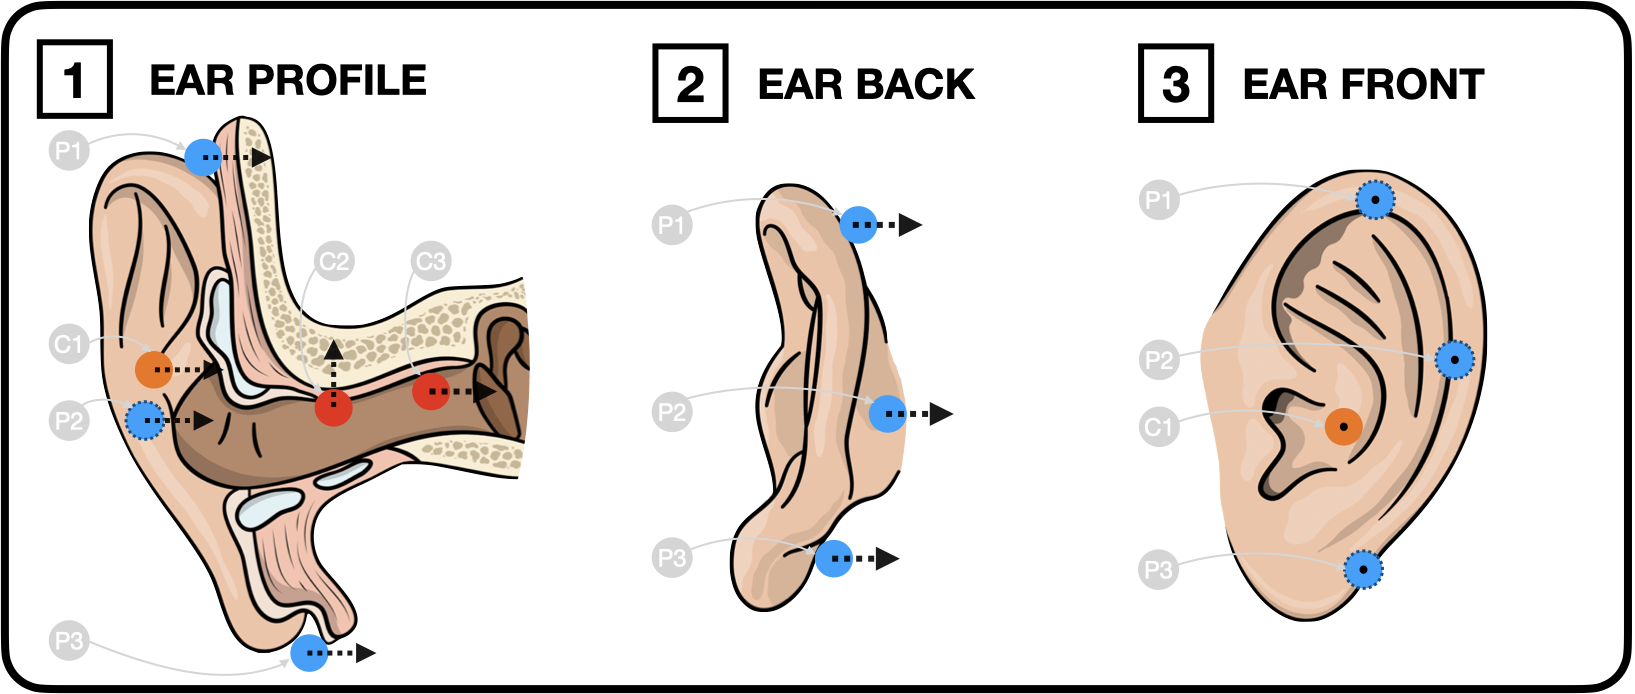
\includegraphics[scale=0.26]{thesis-doc/images/ear_measurement_points/emp.png}
    \caption{Here the temperature measurement points are shown visually from different angles (profile view (1), ear from behind (2), ear from the side (3)). $P1$-$P3$ are three measuring points behind the ear, which measure the skin temperature at the mastoid. $C1$ is a measuring point that measures the temperature at the concha. $C2$ and $C3$ measure the temperature in the ear canal, where $C3$ is directed at the tympanic membrane and $C2$ is directed at the edge of the ear canal. The arrows at each measuring point show the measuring direction. In addition, a measuring point is outlined with a dashed line if it is located behind the ear. The sensor used is the MLX90632, which is an infrared temperature sensor. This is connected to the OpenEarable and the sensor values can be received and persisted using the I2C protocol.}
    \label{fig:ear_measurement_positions}
\end{figure}

\section{Expected Results}
\label{ch:Introduction:ExpectedResults}
The study is expected to provide insights into the placement of sensors for temperature monitoring in or directly on the ear.
Possible variations in temperature measurements at different positions in the ear canal will be identified to adequately detect temperature at the ear in everyday situations.
The results will support the development of more accurate and reliable wearable devices for biometric applications. 
In addition, the optimally determined position will serve as a new basis for the analysis of various body temperature changing events.
The second study, which is being conducted as part of this work, will demonstrate small-scale temperature increases under stress and provide preliminary findings.  % Einleitung
\chapter{Background \& Related Work}
\label{ch:Background}
This chapter first introduces important aspects of body temperature and then sensing with earables.
For body temperature, a distinction is made between core body temperature and skin temperature. 
In addition, the focus is on how temperature can be measured. 
In the subchapter on sensing with earables, the recording of data on the ear is generally introduced. 
Here a division of Röddiger \cite{roddigerSensingEarablesSystematic2022a} is explained.

\section{Body Temperature}
\label{Background:BodyTemperature}
In medical practice, temperature is one of the most frequently measured physical quantities.
By measuring temperature, one gains information about the internal energy of an object.
From the biophysical point of view, temperature measurement determines the changes in physical quantities that occur in a thermodynamic system \cite{dolibogComparativeAnalysisHuman2022}.
Temperature can be expressed in different scales.
These include Celsius, Fahrenheit, Kelvin, and Rankine \cite{grodzinskyUnderstandingFeverBody2020}.
The human body temperature range is usually between $36.5-37.5^\circ C$ \cite{hutchisonHypothermiaTherapyTraumatic2008}, varies constantly and depends on many influencing factors such as gender, age, time of day, and many others \cite{sund-levanderNormalOralRectal2002}.
Likewise, the state of consciousness and emotions are a decisive factor that significantly influences the body temperature \cite{barbosaescobarTemperatureEmotions2021}.
Furthermore, the position at which body temperature is measured is crucial \cite{Physiologie9783137960072ZVAB}.
In order to keep the body temperature within the normal temperature range through internal and external factors, the body uses thermoregulation, through which the temperature is constantly adjusted by signals from the central nervous system.

\subsection{Thermal Regulation}
\label{Background:BodyTemperature:ThermalRegulation}
A vital body function is the possibility of regulation of the exchange of body heat \cite{grodzinskyUnderstandingFeverBody2020}.
Regulation occurs through a neural feedback system. 
In many body parts, sensory means detect cold and heat and transmit them via the central nervous system to the hypothalamus reacting to potential temperature adjustments by triggering physiological activity. 
This can be associated with a gain or loss of heat, which maintains body temperature.
Major players in regulating body temperature are the cardiovascular system, the sudomotor control system, and skeletal muscles. 
The goal is to maintain body temperature within the range of $35^\circ C$ to $41^\circ C$ \cite{pierauTemperatursensibilitaet2001}. 
An excessive increase in body temperature (hyperthermia or hyperpyrexia), in which temperature regulation is no longer working, must be treated as a medical emergency.
The same applies if the body temperature drops below $35^\circ C$.

\subsection{Core Body Temperature}
\label{Background:BodyTemperature:CBT}
Core body temperature is the temperature of the body's internal organs, such as the heart, liver, and brain, and is a commonly used indicator of human health and endurance performance.
Unlike the body core temperature, the body surface temperature is more easily influenced by the ambient temperature and therefore cannot reflect the changes inside the body as well as the body core temperature.
Core body temperature can be measured invasively rectally, orally (oesophagus), in the pulmonary artery (with the use of a catheter), or in the urinary bladder \cite{moranCoreTemperatureMeasurement2002a}.
However, the gold standard is different.
The core body temperature of a healthy human body differs almost little from the temperature of the blood flowing in the pulmonary artery \cite{krizanacFemoroiliacalArteryPulmonary2013, holtzclawMonitoringBodyTemperature1993}.
This is exactly what is used as the gold standard for measuring body core temperature \cite{krizanacFemoroiliacalArteryPulmonary2013, holtzclawMonitoringBodyTemperature1993, fulbrookCoreBodyTemperature1997, maxtonEstimatingCoreTemperature2004}.
However, this comes with a few critical points.
Measuring the temperature of the blood flowing in the pulmonary artery involves an invasive and risky procedure that requires the insertion of a pulmonary artery catheter \cite{yeohRevisitingTympanicMembrane2017}.
This is strongly recommended in a medical hospital and nowhere else.
All of the previously mentioned methods are not comfortable for humans when measuring over a long period of time in everyday life.

Body temperature can also be measured non-invasive.
The following methods are much more convenient, but the measurement accuracy suffers somewhat.
Measuring the body temperature non-invasive can be done on the axilla, the tympanic membrane, and the body surface \cite{moranCoreTemperatureMeasurement2002a}.
Usually, core body temperature is constant only in the body core and consequently cannot be determined outside only by temperature sensors \cite{niedermannPredictionHumanCore2014}.
Due to this, it is necessary to use several other values for the calculation of the core body temperature in order to approximate the true temperature value. 
These can include e.g. skin temperature and skin heat fluxes or the heart rate.
Niedermann achieved a root mean square deviation (rmsd) ranging from $0.28 ^\circ C$ to $0.34 ^\circ C$ for all environmental conditions in 2014 \cite{niedermannPredictionHumanCore2014}.
Therefore, a principal component analysis (PCA) was performed to extract uncorrelated variables that were subsequently used in a linear regression model. 
Six parameters, consisting of three skin temperatures, two skin heat currents, and heart rate, were selected as input variables to generate two principal components. 
The predictive power of these components for estimating core body temperature was evaluated using multiple regression analysis.

\subsection{Skin Temperature}
\label{Background:BodyTemperature:SkinTemperature}
Skin temperature is often used to measure body temperature.
Skin temperature in general is the result of a dynamic equilibrium between the heat released during metabolic processes and transferred to the skin layer by thermal conduction and convection, the heat extracted from the environment, and the heat transferred to the environment by radiation, convection, and evaporation \cite{dolibogComparativeAnalysisHuman2022}.
Various sensors are used to measure skin temperature. 
These include the infrared sensors, but also the thermistors. 
Both are equal for purposes of clinical electrodiagnostic readings.
Thermistors offer better responsiveness and sensitivity in measurements.
Infrared thermistors, on the other hand, are more convenient in terms of speed and maneuverability \cite{burnhamThreeTypesSkinSurface2006}.
Because the skin is exposed to external influences, temperature differences can quickly occur.
This can be caused by cold or warm ambient air, but also by rain or other influences.
Measurements on the skin that cannot be easily influenced, such as the armpits, are suitable here.

\subsection{Temperature Measurements}
\label{Background:BodyTemperature:TemperatureMeasurements}
% TODO: General Temperature measurements of the human body
In General, the temperature of a human body will be measured with a thermometer.
There are multiple techniques available on which the temperature value will be calculated. 
These are divided into contact and non-contact thermometers.
For a detailed overview, take a look at chapters \ref{Background:TemperatureSensors:OpticalTS} and \ref{Background:TemperatureSensors:ResistanceTD}.
Body temperature is often measured in the armpit, mouth, rectum, ear, or forehead.
The temperature in the armpit is typically $36.6^\circ C$, in the mouth $36.9^\circ C$, and $37.1^\circ C$ in the ear \cite{dolibogComparativeAnalysisHuman2022}.
% TODO: wie siehts bei Rectal aus?
The rectal temperature testing method is the most accurate of all measurements, while non-contact forehead thermometers are considered the least accurate, and measurements are taken with them should be confirmed by other methods.
The minimum value of the standard error for the above methods is $0.1^\circ C$ [9].
Ear readings are assumed to be of similar accuracy when compared to the rectal method, which is most commonly used in infants, the correct value is usually $37.1^\circ C$ \cite{dolibogComparativeAnalysisHuman2022}.

% Ear based temperature measeurements
Ear-based temperature measurement uses a sensor to measure the temperature of the ear canal. 
The approach has a number of advantages over other measurement positions.
First, it is a non-invasive measurement procedure, which allows measurement nearly inside the body with the least amount of hematoma.
Second, the measurement is much more promising compared to other non-invasive alternatives, where many factors can contribute to falsifying the final result \cite{ganioValidityReliabilityDevices2009, craigTemperatureMeasuredAxilla2000}. 
However, it is essential to note that the accuracy of temperature measurement may depend on factors such as the positioning of the thermometer and the presence of earwax or other obstructions in the ear canal.

% \subsubsection{Temperature Measurements on the Tympanic Membrane}
The tympanic membrane is a thin membrane that separates the middle ear from the external auditory canal. 
The artery called the external carotid artery runs near the external auditory canal and radiates heat, which is why measuring the temperature at the tympanic membrane has a promising chance of determining body temperature \cite{yeohRevisitingTympanicMembrane2017}.

Since measuring body temperature at the tympanic membrane is a non-invasive measurement method, it is already being investigated as a possible replacement for currently accepted methods.
This could be a safe and very convenient way of measuring core body temperature, but to date it is not de-facto due to unresolved problems.
These include the accuracy and stability compared to measurements at other locations \cite{maxtonEstimatingCoreTemperature2004, fulbrookCoreBodyTemperature1997, mumaComparisonRectalAxillary1991, rothAgreementRectalTympanic1996}.
Benzinger \cite{benzingerHeatRegulationHomeostasis1969, benzingerClinicalTemperatureNew1969, benzingerPhysicalHeatRegulation1959} first demonstrated the feasibility of tympanic membrane measurement as an indicator of core body temperature using a thermocouple temperature probe that engages the surface of the tympanic membrane with the ear canal sealed from the environment.
For this, Benzinger made measurements of tympanic membrane temperature obtained from his probe and measurement approach and showed them to be stable, reproducible, and responsive to thermal stresses of various types.
However, there are other studies at a later date that refute individual assumptions of this study.
McCaffrey et al. \cite{mccaffreyEffectHeadSkin1975} and Nielsen \cite{nielsenNaturalCoolingBrain1988} showed that head cooling reduces the body core temperature when measured with exactly the procedure of Benzinger.
McCaffrey et al. however, also showed that by heating and cooling localized regions of the head, infrared measurement of temperature at the tympanic membrane of human subjects was not proportionally affected by changes in head skin temperature.
This suggests a contradiction, which means that this method may not be a good predictor of core body temperature because it depends on other, as yet unknown, variables.
Brinnel and Cabanac \cite{brinnelTympanicTemperatureCore1989} and Sato et al. \cite{satoReexaminationTympanicMembrane1996}, however, provided data showing that measurements for this purpose are still reliable if the measurement point on the tympanic membrane is carefully chosen. 
Brinnel and Cabanac proposed that the lower anterior quarter of the tympanic membrane (Figure \ref{fig:tympanic_membrane_mp}) has a higher temperature on the surface of the tympanic membrane and temperature measurement from a point in this area is the least sensitive to head cooling.
\begin{figure}[t]
    \centering
    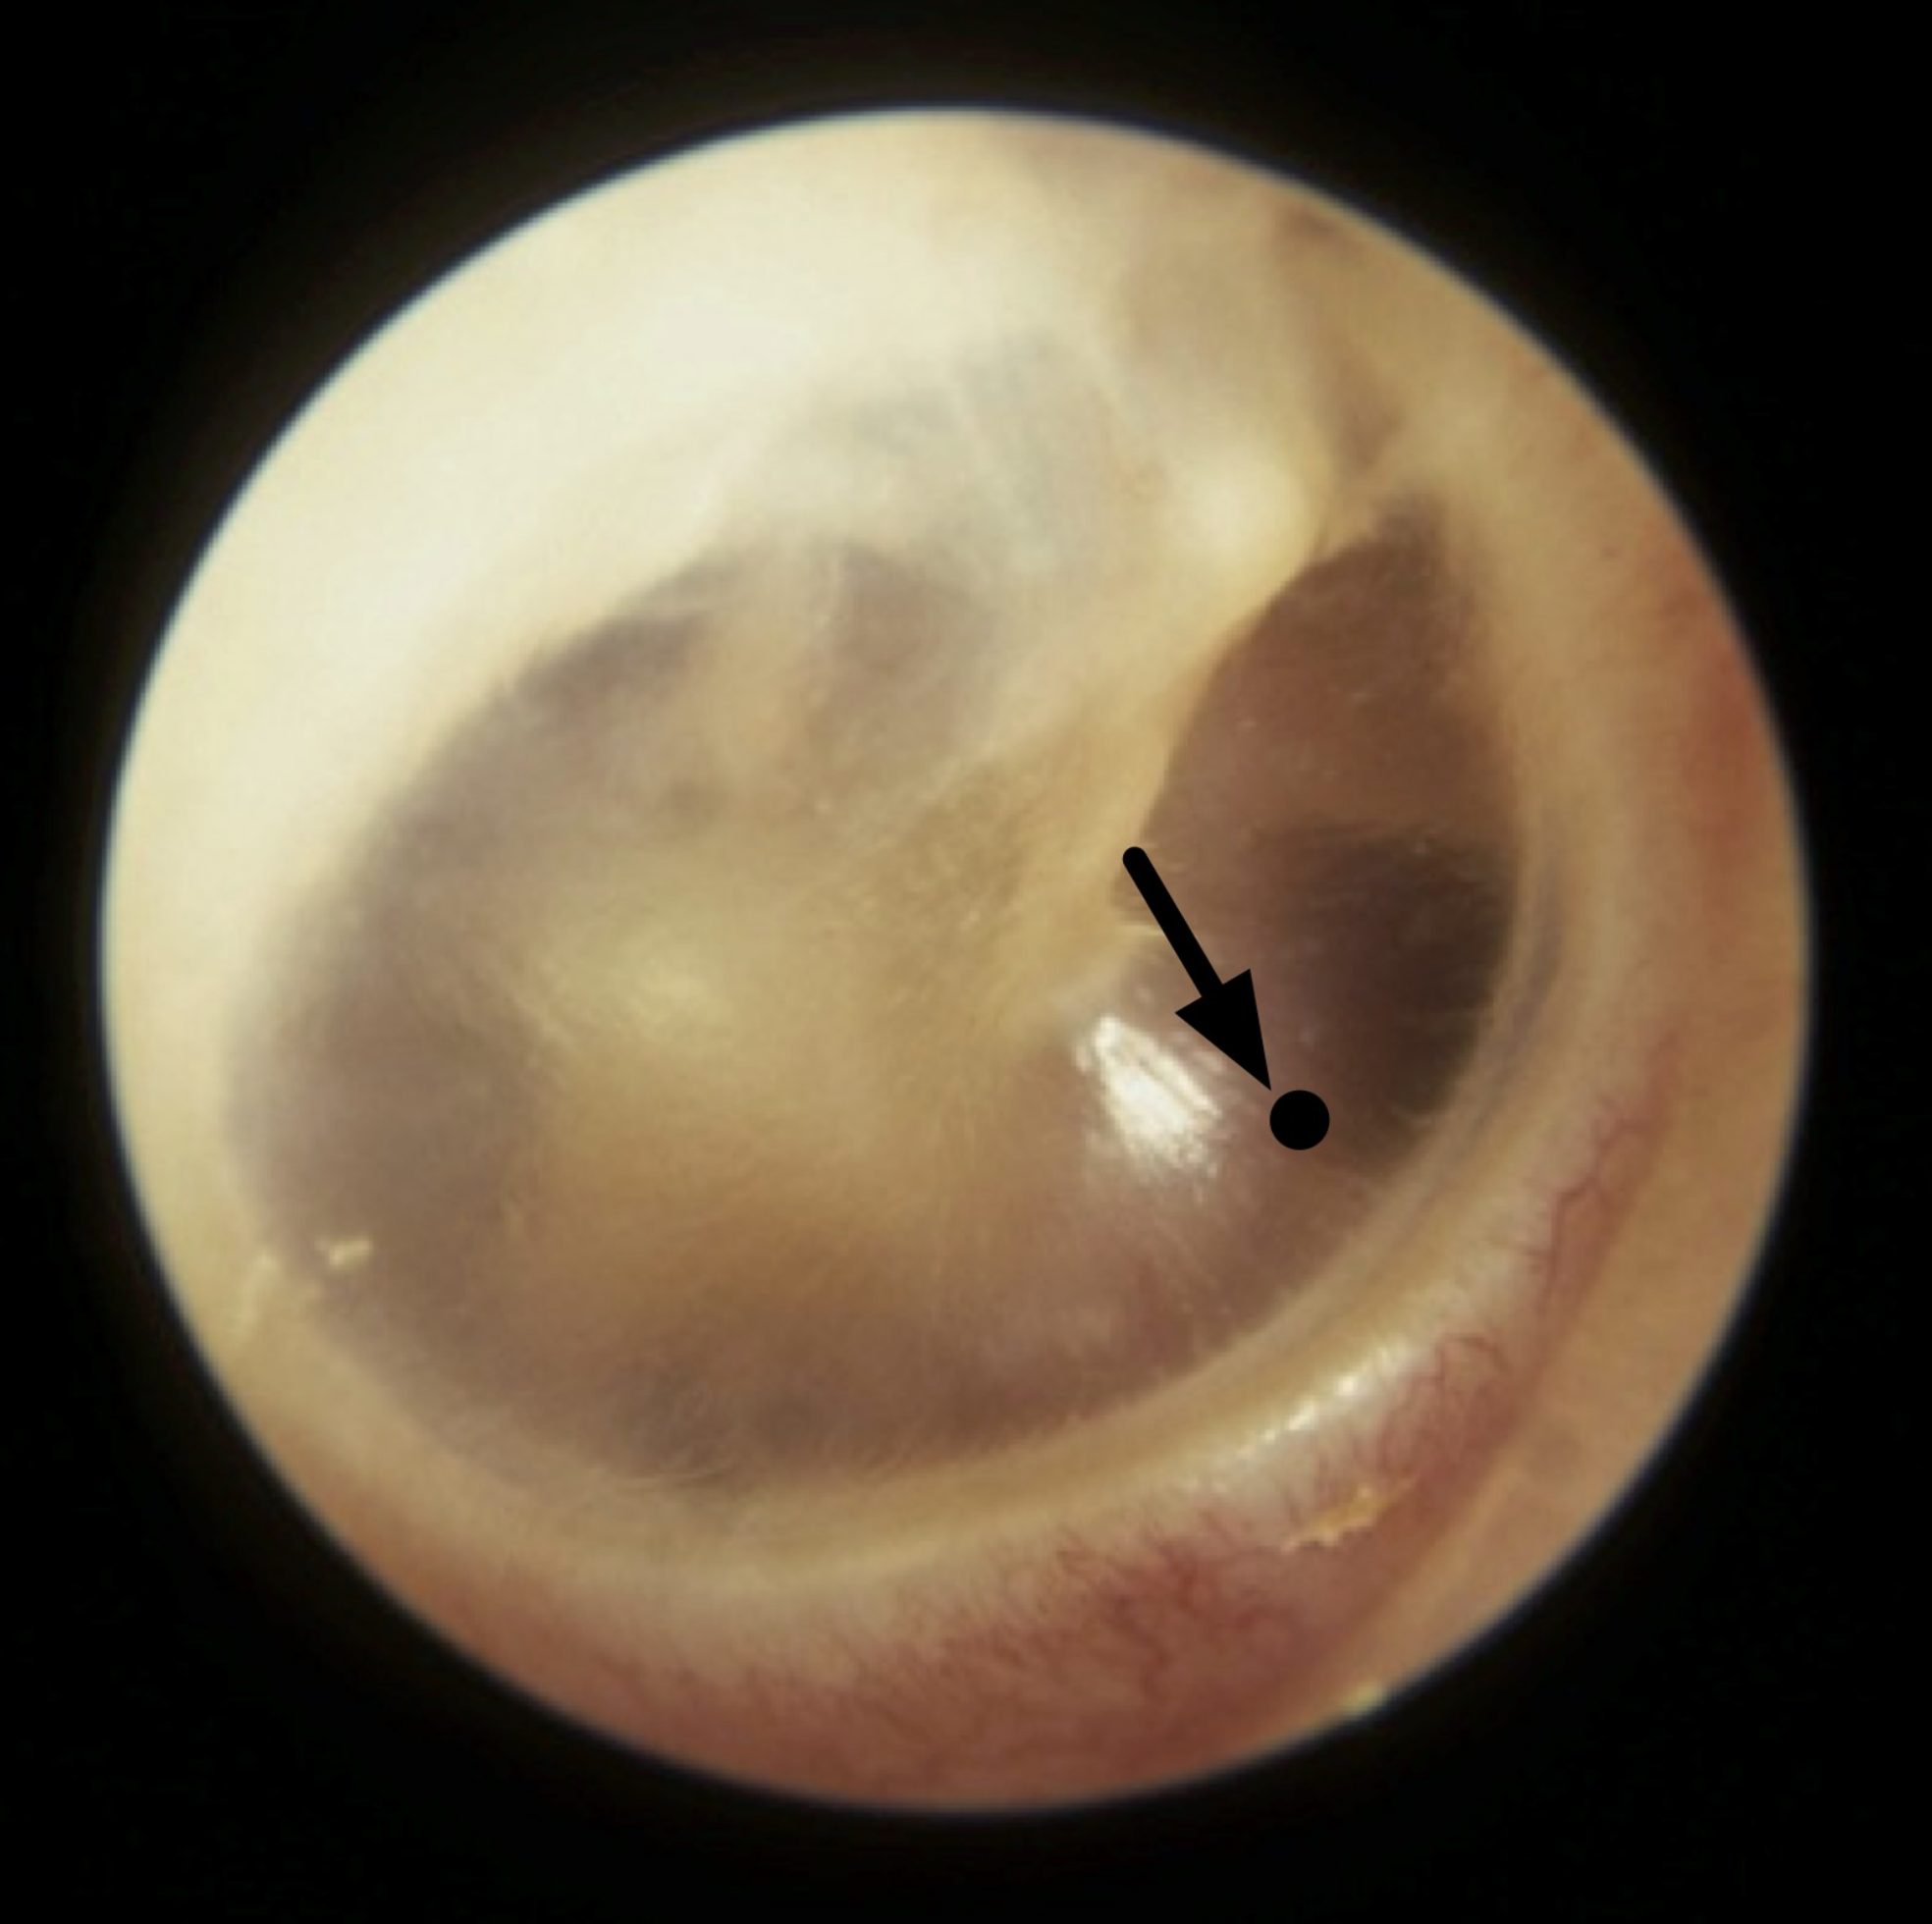
\includegraphics[scale=0.15]{thesis-doc/images/tympanic_membrane_mp.png}
    \caption{Measuring point on the tympanic membrane \cite{brinnelTympanicTemperatureCore1989}. Tympanic membrane of the right ear with a temperature measuring point in the lower front quarter (see arrow).}
    \label{fig:tympanic_membrane_mp}
\end{figure}

% das paper is von 1991, vllt schon zu alt und unrelevant
% TODO: \cite{ComparisonPulmonaryArtery}

% hier bei der comparison gehts um mittelohrentzündungen
% TODO: \cite{kimComparisonBilateralEardrum2022}

% das paper is von 1999, vllt schon zu alt und unrelevant
% TODO: \cite{childsTympanicMembraneTemperature1999}

Temperature sensors are used to measure the temperature of a particular object or environment.
They are widely used in many applications, such as industrial, medical, or scientific contexts.
Temperature sensors detect changes in temperature and convert this into a measurable signal.
There are various types of temperature sensors, including contact and non-contact sensors.
% Contact sensors
Contact sensors measure temperature by maintaining physical contact with an object and measuring the temperature there.
Contact sensors can be divided into 3 types: Thermocouples, Thermistors, and Resistance Temperature Detectors (RTDs). 
Thermocouples measure the voltage generated by two different metals when they are exposed to different temperatures.
RTDs measure changes in the electrical resistance of a metal wire when it has temperature changes.
Thermistors are semiconductor devices whose electrical resistance changes with temperature.
% Non-contact sensors
Non-contact sensors, on the other hand, do not require contact with the object being measured. They are also known as infrared sensors.
Non-contact sensors measure the emitted infrared radiation from an object and convert it into a measurable signal.
Most often, the sensors are used when contact with an object is not desirable or practical, such as can often be useful in a medical or scientific research context. 
This is also the case in this work, as contact with the tympanic membrane, for example, is not desired.
Non-contact sensors can be roughly divided into two categories: IR sensors and optical pyrometers.
IR sensors are devices that detect and measure the amount of infrared radiation emitted by an object. They operate on the principle that all objects emit infrared radiation in proportion to their temperature. 
Optical pyrometers, on the other hand, measure temperature by detecting the color of light emitted by an object. They work on the principle that the color of light emitted from a hot object changes as the temperature of the object changes.
However, the current classification here is very crude.
In addition to those mentioned above, there are, for example, fiber optic sensors and acoustic sensors.

When choosing the right sensor for a particular application, some things have to be considered.
Accuracy, response time, and range are important variables.
Depending on the requirement profile, the right sensor can be selected based on the parameters.
In the following, the optical temperature sensors, as well as the RTDs are described in more detail, since they are very important in this work.

\subsection{Optical Temperature Sensors}
\label{Background:TemperatureSensors:OpticalTS}
Optical temperature sensors, also known as optical pyrometers, measure temperature by detecting the color of light emitted from an object. 
This is based on the assumption that the color of the emitted light is different depending on the temperature.
Typically, this is done using a lens that focuses the emitted light from the object onto a detector, which then analyzes the color of the light. 
This is then ultimately used to determine the temperature.
This type of sensor is typically used in applications where contact with the object being measured is difficult or impossible, such as in space, harsh environments, or just where contact is not wanted.
Thus, non-contact measurements are possible, which is essential when measuring the temperature of the tympanic membrane.
Another advantage of optical temperature sensors is that moving objects can still be measured as long as the sensor continues to point at the object.
However, this requires a line of sight to the measured object.
In addition, accuracy can be affected by reflective surfaces or atmospheric conditions, which should not be a problem if the measurement is primarily in the ear.

\subsubsection{MLX}
\label{Background:TemperatureSensors:OpticalTS:MLX}
The MLX90632 sensor is an infrared thermopile temperature sensor.
It measures temperature without requiring contact with the skin. 
This is done by means of an infrared sensor. 
The sensor is based on a microelectromechanical system (MEMS), which is used to detect thermal radiation in the infrared spectrum emitted by the object to be measured \cite{melexisMLX90632FIRSensor2021}.
The MLX90632 has a small form factor and low power consumption, which is well-suited for small devices.
In addition, the sensor has a very high accuracy of $\pm 0.5 ^\circ C$ from $-20 ^\circ C$  to $100 ^\circ C$.
Here the sensor can resolve in $0.02 ^\circ C$ steps.
Another immense advantage is the simultaneous measurement of 2 temperature values at the same time.
This is possible because 2 sensor elements are directly installed in the MLX90632.
This enables the measurement of one object, such as the skin temperature, and the ambient temperature.
However, it is also possible to measure 2 different body parts at the same time.
In order to be able to integrate the sensor optimally into a system, an I2C interface is available so that a microcontroller can communicate easily.
Overall, the MLX90632 sensor provides a versatile and accurate solution for non-contact temperature measurement in a variety of applications, including medical, industrial, and consumer electronics.

\subsection{Thermal Resistance Temperature Detectors}
\label{Background:TemperatureSensors:ResistanceTD}
Thermal resistance temperature detectors operate by measuring changes in electrical resistance as a function of temperature. 
This type of sensor is typically used in applications where high accuracy is required, such as laboratory environments or medical equipment.
They provide high accuracy and cover a wide range of temperature measurements.
However, contact measurement is required here, which limits temperature measurement to stationary objects.
Furthermore, thermal resistance temperature sensors have a slow response time, which makes real-time measurement somewhat difficult.

In summary, optical temperature sensors are useful in situations where contact with the object being measured is difficult or impossible, while thermal resistance sensors are suitable for applications that require high accuracy and a wide temperature measurement range. 
Ultimately, the choice between these two types of sensors depends on the specific requirements of the application.

Here in the master's thesis, optical temperature sensors are suitable because they do not require direct contact points, which is essential when measuring temperature on the tympanic membrane.

\subsection{Stress and Its Effects on Body Temperature}
Stress is a physiological and psychological response to either challenging tasks or threatening situations \cite{jamesUnderstandingRelationshipsPhysiological2023}. 
Stressors can be acute or chronic.
An acute stressor, such as a near-accident with a car), directly elicits a stress response, which, however, subsides immediately after its occurrence.
A chronic stressor, on the other hand, lasts for a longer period of time. 
These include, for example, financial problems or persistent illness.
Here there are no quick solutions and the problems are less quickly forgotten \cite{baumControlIntrusiveMemories1993}.
Stress can have positive and negative effects.
On the one hand, stress can lead to rising above oneself in dicey situations, but in excessive or prolonged stressful situations it can negatively affect one's mental and physical condition \cite{jamesUnderstandingRelationshipsPhysiological2023}.
In this regard, prolonged stress can cause, for example, digestive and gastrointestinal problems, hypertension, diabetes, cardiovascular disease, bone mineral loss, immunosuppression, and asthma \cite{merabetHowExposureChronic2022, dhamaBiomarkersStressRelated2019, petriePrevalencePTSDCommon2018}.

Stress activates the body's fight-or-flight mechanism, which leads to various physiological changes, including an increase in body temperature \cite{marazzitiPsychologicalStressBody1992}. 
This chapter focuses on the effect of stress on body temperature. 
This is to provide the scientific basis a study of stress detection through temperature measurements at the ear.
The human body's response to stress is complex and involves multiple systems, including the endocrine system, the nervous system, and the immune system \cite{jamesUnderstandingRelationshipsPhysiological2023}. 
One of the immediate physiological responses to stress is hyperthermia, a transient increase in core body temperature \cite{vinkersEffectStressCore2013}. 
This phenomenon is part of the body's acute stress response, often referred to as the fight or flight response \cite{vinkersEffectStressCore2013}.
The increase in body temperature during stress has already been shown in several studies.
In a study by Nakata in 2021, a passive heat stress test was conducted and found to result in an increase in internal temperature of approximately $1.2 ^\circ\text{C}$ and to impair cognitive function \cite{nakataEffectsPassiveHeat2021}. 
This study suggests that heat stress may have a significant impact on neuronal activity related to cognitive function.
In another study, subjects were inflicted stress using the Trier Social Stress Test (TSST) \cite{vinkersEffectStressCore2013}. 
Here, subjects had to perform a 5 minute with a preparation time of 3 minutes job interview in front of a committee with a microphone. 
In addition, mental arithmetic tasks were subsequently performed. 
The subject was told at the beginning that everything would be video recorded.
In this study, an increase in heart rate, an increase in skin temperature, and an increase in respiration rate were detected, among others. 
% ADD CONTENT

\section{Sensing with Earables}
\label{Background:SensingWithEarables}
Earables belong to the class of wearables and are a type of wearable device that is worn in or around the ears. 
They typically have a number of sensors that allow them to collect data about the wearer's physiology and activity. 
The most common sensors in earables include accelerometers, gyroscopes, and heart rate monitors. 
These sensors can be used to track the wearer's movements, monitor their heart rate, and provide other types of health data.
Earables are portable, lightweight, and small, which allows them to be worn easily for long periods of the day \cite{roddigerSensingEarablesSystematic2022a}. 
Thus, data can be tracked over a longer period of time. In addition, earables have the advantage of being worn on the ear, which together with the head are automatically stabilized during movements and thus have less motion disturbances and artifacts \cite{grossmanFrequencyVelocityRotational1988, kavanaghRoleNeckTrunk2006a}.
% Why the position of the ear is important
The position on the ear provides a lot of potential. 
For one thing, the ear is very close to the brain and blood vessels, which allows accurate measurement of brain activity, cyclic blood flow, and related properties \cite{ferliniInEarPPGVital2022}.
In addition, it is possible to detect the perception of a variety of facial, neck, and eye muscle activations \cite{andoCanalSenseFaceRelatedMovement2017}, as well as the input of head movements \cite{andoCanalSenseFaceRelatedMovement2017}, facial gestures \cite{matthiesEarFieldSensingNovelInEar2017}, mouth movements \cite{sunTeethTapRecognizingDiscrete2021a}, and instantaneous \cite{bleichnerConcealedUnobtrusiveEarCentered2017, phamWAKEBehindtheearWearable2020}. 
Because of the ease of accessibility with the hand \cite{kikuchiEarTouchTurningEar2017, xuEarBuddyEnablingOnFace2020}, interactions with the hand on the ear can be used to trigger actions \cite{lissermannEarPutAugmentingEarworn2014}.
In summary, earables are capable of triggering a variety of processes of the skeleton (e.g., gait \cite{atallahGaitAsymmetryDetection2014}), muscles (e.g., facial expressions \cite{matthiesEarFieldSensingNovelInEar2017}), nerves (e.g. Brain activity \cite{debenerUnobtrusiveAmbulatoryEEG2015}), endocrine system (e.g., emotions \cite{athavipachWearableInEarEEG2019}), cardiovascular system (e.g., blood pressure \cite{atallahValidationEarwornSensor2012}), respiratory system (e.g., breathing \cite{roddigerRespirationRateMonitoring2020}), and digestive system (e.g., food intake \cite{gaoIHearFoodEating2016}).

In 2022, Röddiger et al. noted the current state of research on sensing with earables \cite{roddigerSensingEarablesSystematic2022a}.
A systematic literature review of 271 peer-reviewed research articles was made receiving a better understanding of the current state of research on this topic.
The research area was divided there into four categories (Figure \ref{fig:sensing_with_earables_overview}), which will now be explained in more detail.

\begin{figure}[t!]
    \centering
    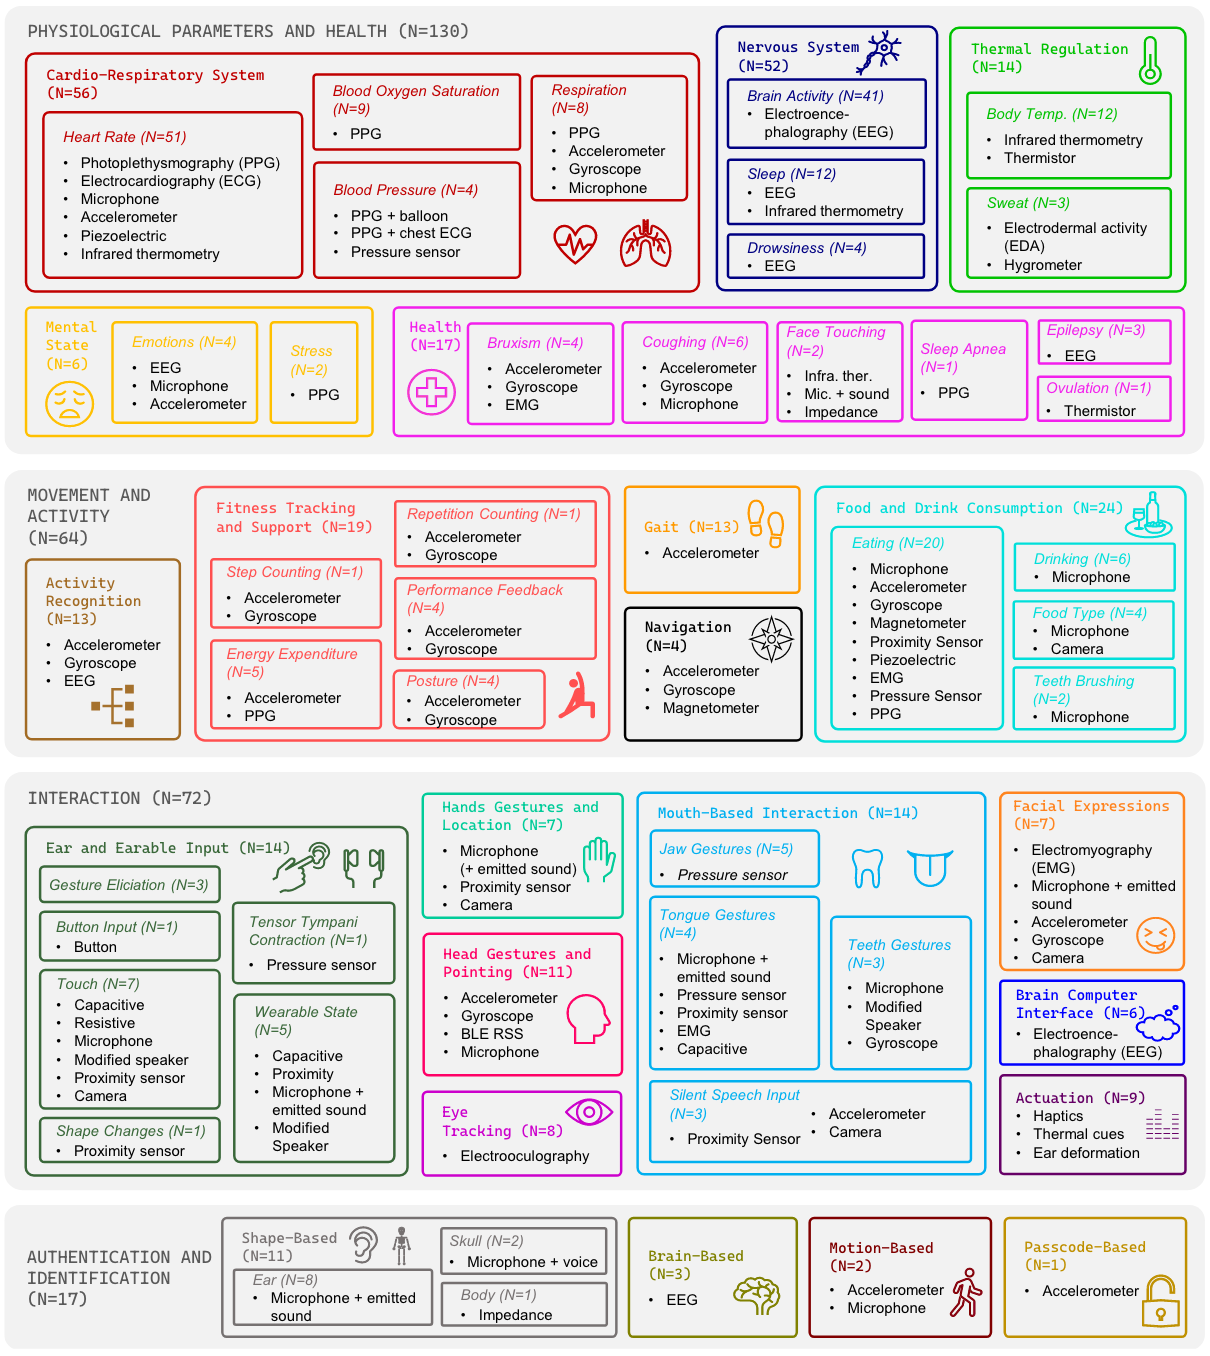
\includegraphics[scale=0.3525]{thesis-doc/images/sensing_with_earables_overview.png}
    \caption{Overview map of sensing with earables. The map displays all phenomena current research is about divided into the main four categories. For each phenomena, there is a number (N), which describes the available articles and all the used sensors used to detect these phenomena \cite{roddigerSensingEarablesSystematic2022a}.}
    \label{fig:sensing_with_earables_overview}
\end{figure}

\subsection{Physiological Monitoring and Health}
\label{Background:SensingWithEarables:Physiological}
The first categorical classification of sensing with earables is physiological parameters and health \cite{roddigerSensingEarablesSystematic2022a}.
The use of ear-worn sensors to track and maintain personal health by monitoring various physiological parameters is considered.
The parameters are categorized according to human body functions such as the cardio-respiratory system, nervous system, thermoregulation, mental status, and health monitoring.
The cardio-respiratory system is divided into the areas of heart rate, blood oxygen saturation, respiration, and blood pressure.
All these areas can be classified, for example, with a PPG (photoplethysmography). 
When determining the heart rate, a microphone, an accelerometer, an infrared thermometer, the piezoelectric, or an EEG (electrocardiography) can be used.
The nervous system includes the classification of brain activity, sleep, or drowsiness. 
All are determined using an EEG. When classifying sleep, an infrared thermometer can also be used for classification. 
The most researched area here in the context of earables is brain activity.
The third subcategory in the physiological parameters and health represents the mental state.
This has not yet been researched that far in the context of earables with 6 reference papers.
Emotions can be recognized using an EEG, a microphone, or an accelerometer, and even stress using a PPG.
Another subcategory is health which is divided into bruxism, coughing, face touching, sleep apnea, epilepsy, and ovulation.
Sensors such as an accelerometer, a gyroscope, a microphone, an EEG, PPG, or an infrared thermometer are used here.
For further details please refer to the original paper \cite{roddigerSensingEarablesSystematic2022a}.
The last part of the physiological parameters and health is thermal regulation. A distinction is made here between body temperature and perspiration. An EDA (electrodermal activity) and a hygrometer are used for sweating.
When classifying body temperature, an infrared thermometer, and a thermistor are used.
Due to the body temperature being the most crucial part of this thesis, this part will now be focused in more detail.

\paragraph{Body temperature}
\label{Background:SensingWithEarables:Physiological:BodyTemperature}
Bestbier and Fourie \cite{bestbierDevelopmentVitalSigns2018} applied the principle to a wearable form factor and achieved a small mean error of only $0.02$ $\pm$ $0.52 ^\circ C$. 
They used the TMP006 infrared sensor, which points directly at the tympanic membrane. 
The thermophilic voltage and the temperature sensor were made digitally available via hardware registers, from which the object temperature can be calculated. 
This reflects the temperature of the tympanic membrane after calibration.
However, the accuracy varies greatly between individual positions, which is attributed to the orientation of the sensor due to a wide variety of auditory canals.
This problem was solved by implementing intraparticipant calibration.
This should allow the sensor to self-calibrate automatically and improves the standard error by $56\%$ (from $0.5125 ^\circ C$ to $0.29 ^\circ C$) and the correlation coefficient from $0.4667$ to $0.8684$.

However, user-defined calibration is needed because the shape of the ear canal is different for each individual \cite{bestbierDevelopmentVitalSigns2018, luekenPhotoplethysmographybasedInearSensor2017, matsumotoEarbudtypeWearableHearable2019}.
Luken et al. integrated TI's TMP007 into the proposed measurement system to obtain information about human core temperature variation at a rate of $33 Hz$ \cite{luekenPhotoplethysmographybasedInearSensor2017}.
For individual calibration purposes, the voltage difference of the thermopile element and the chip temperature was transmitted in addition to the recorded object temperature.
However, the temperature was not further calibrated or processed in this work \cite{luekenPhotoplethysmographybasedInearSensor2017}.
Alternatively, surface skin temperature at the mastoid can be determined with high accuracy ($0.03 ^\circ C$ mean error) \cite{atallahErgonomicWearableCore2018}.
% TODO: read atallahErgonomicWearableCore2018 paper and insert content
A known factor for changes in body temperature is considered in earable research to be the response to external weather conditions \cite{barralonAugmentedHearingAssistance2015, boanoNoninvasiveMeasurementCore2013, celikEvaluationBehindtheEarECG2016} and during physical activities \cite{boanoNoninvasiveMeasurementCore2013, chagllae.MeasurementCoreBody2018, celikEvaluationBehindtheEarECG2016, matsumotoEarbudtypeWearableHearable2019, sugimotoDevelopmentWirelessSensing2011}.
% TODO: read all the previous papers and explain a lot more here!
These findings enable a number of applications that perform some important functions, such as alerting or vital signs and parameter tracking based on the identified relationships.
In addition, the relationship between body temperature recorded at the ear and ovulation (see subsection 4.5.6) and sleep (see subsection 4.2.2) has been demonstrated.
% TODO: remove the above sentence and insert content from sections mentioned

\subsection{Movement and Activity}
\label{Background:SensingWithEarables:Movement}
Another categorical classification of sensing with earables is movement and activity \cite{roddigerSensingEarablesSystematic2022a}.
Here, the focus is on detecting user movements and deriving insights about activities performed by the user. 
Movements detected at the ear can be classified into discrete classes, such as a user's posture, their movement, and also the type of activity. 
Beyond simply classifying sensor data, the project also explored how physical quantities can be derived from the user's movement to provide useful information for a variety of applications, including fitness tracking, gait analysis,
food and beverage consumption, and inertial navigation.
Most of the findings are recorded with the accelerometer and the gyroscope.
Activity recognition is recognized with it, but also with an EEG. Accelerometers and gyroscopes are also used as a basis for the fitness tracking and support subcategory, and the EEG for sensor performance.
When measuring the gait, the signal from the accelerometer is sufficient.
Significantly more sensors are used for classification when eating. While only one microphone signal was used for the drinking detection, a series of signals is used for the eating detection. 
Here the microphone, accelerometer, gyroscope, magnetometer, proximity sensor, piezoelectric, EMG, pressure sensor, and also the PPG is used.
When brushing teeth is detected, a microphone signal is evaluated.
In addition, the accelerometer and gyroscope signal as well as a magnetometer are also used for navigation.

\subsection{Interaction}
\label{Background:SensingWithEarables:Interaction}
Interaction is another categorical classification of sensing with earables \cite{roddigerSensingEarablesSystematic2022a}.
Since earables have a lot of different sensors, there are exciting possibilities for unique and novel interactions.
So far, attempts have been made to recognize inputs on the ear, but also on other parts of the body that can be recognized by sensors on the ear.
Subfields of interaction include ear or earable input, hand gestures or hand position, head gestures or orientations, eye tracking, mouth-based tracking, facial expressions, brain-computer interface, and actuation.
The most common tracking techniques are pressure or proximity sensors, accelerometer and gyroscope, the microphone, and EEG and EMG.
There are various input options for the ear-based or earable-based input. These include button inputs, touch or shape changes, and others.
Mouth-based interactions can be divided into jaw activities, tongue gestures, tooth activities, and silent speech input.

\subsection{Authentication and Identification}
\label{Background:SensingWithEarables:Authentication}
The final categorical classification of sensing with earables is authentication and identification \cite{roddigerSensingEarablesSystematic2022a}. 
For secure access to sensitive data, mobile devices often use biometrics such as fingerprints. 
Earable technologies have explored biometric authentication based on the unique ear, skull, or body features, as well as brain activity and body movement. 
Passcode-based authentication methods that use rhythmic patterns have also been proposed. 
The two main approaches are verification and identification, where performance is often measured using an equal error rate (ERR) to balance false acceptance and false rejection rates.
In this categorical classification, the microphone and emitted sound are used as the basis in shape-based authentication and identification on the ear, the microphone and voice are used in the skull, and impedance is used in the body.
The EEG is the basis for recognition in brain activity-based authentication and identification.
When the individual movement is used for authentication and identification, the accelerometer and the microphone are used, in the passcode-protected authentication and identification only the accelerometer signal is used.

\subsection{Sensing Platforms}
\label{Background:SensingWithEarables:SensingPlatforms}
Ear-based sensing platforms have gained considerable attention in the wearable technology field due to their potential for multiple applications and benefits. 
This chapter examines different types of ear-based sensor platforms, discusses their technical aspects and characteristics, captures their application, and examines the challenges and future directions in this field.
One type of ear-based sensor platform is the in-ear sensor, in which sensors are placed directly in the ear canal. Examples of in-ear sensors are earphones with integrated sensors that can monitor various physiological parameters \cite{maseHearablesNewPerspectives2020, bestbierDevelopmentVitalSigns2018, luekenPhotoplethysmographybasedInearSensor2017}. 
Another type is the on-ear sensor, which is placed on the outer ear or earlobe. 
These sensors can be in the form of clip-on devices or wearable ear accessories to collect specific data.
Behind-the-ear sensors represent another category of ear-based sensor platforms \cite{phamWAKEBehindtheearWearable2020, gilSmartWirelessEarWorn2019, biWearableSensorEating2017}.
These sensors are positioned behind the ear and are often found in hearing aids or smart ear tags. 
Finally, there are ear-worn wearables, which are wearable devices designed to be worn on the ear \cite{biWearableSensorEating2017, gilSmartWirelessEarWorn2019}. 
These include smart earbuds or earbuds that have sensors to monitor various health and activity-related metrics.
Technical aspects and features play a critical role in ear-based sensor platforms. 
Sensor technologies vary by platform, and each has its own advantages and limitations.
Connectivity and data transfer methods are essential for seamless integration with other devices or networks \cite{perezRecentAdvancesWearable2021}. 
Power management strategies are used to optimize battery life and ensure the longer use of ear-based sensor platforms \cite{nguyenInearBiosignalRecording2016}.
Ear-based sensor platforms find applications in various fields. 
In the area of health and wellness monitoring, these platforms enable the tracking of vital signs such as heart rate and body temperature \cite{roddigerRespirationRateMonitoring2020, atallahErgonomicWearableCore2018, maseHearablesNewPerspectives2020, rajbhandaryFeasibilityContinuousMonitoring2020a}.
They also facilitate the monitoring of sleep quality, stress levels, and other health-related parameters \cite{luekenPhotoplethysmographybasedInearSensor2017, wendtThermoregulationExerciseHeat2007}. 
In human-computer interaction, ear-based sensor platforms can serve as input modalities for gesture recognition or control interfaces, making them suitable for augmented reality, virtual reality, and gaming environments. 
In addition, ear-based biometrics are being explored for biometric identification and secure authentication purposes, offering an alternative to traditional authentication methods \cite{roddigerSensingEarablesSystematic2022a}.
Despite the potential benefits, ear-based sensor platforms face certain challenges. 
These include ensuring the accuracy and reliability of measurements, addressing convenience and usability concerns, and addressing privacy and data security issues \cite{bockAccuracyNewInfrared2005, roddigerRespirationRateMonitoring2020, bonziAccuracyPeripheralThermometers2016, gasimAccuracyTympanicTemperature2013, amoateng-adjepongAccuracyInfraredTympanic1999a, ericksonComparisonEarbasedBladder1993, chagllae.MeasurementCoreBody2018}. 
Future research and development efforts will focus on overcoming these challenges, exploring new applications, and advancing the capabilities of ear-based sensor platforms.
In summary, ear-based sensor platforms have emerged as promising tools in wearable technology. 
They offer a range of applications, from health monitoring to human-computer interaction to biometric authentication. 
By leveraging the unique properties of the ear, these platforms provide valuable insights and contribute to the advancement of wearable technology as a whole.

\paragraph{Earables: Temperature Measurement}
The research area of ear based temperature probing is not new territory.
% Temperature measurements at the eardrum
As early as 2010, infared tympanic thermometers (IRTTs) were used to compare temperature at the tympanic membrane with a rectal and oral sample \cite{bagleyValidityFieldExpedient2011, basakComparisonThreeDifferent2013, bhanguDetectionManagementHypothermia2010, fogtNoninvasiveMeasuresCore2017, ComparisonTwoMethods, kallmunzerLocalHeadNeck2011, muthInfraredEarThermometry2010, moran-navarroValiditySkinOral2019, leeValidityInfraredTympanic2011, keeneAccuracyTympanicTemperature2015}.
% TODO: write more if I have the time and fun.
% Temperature measurements outside the ear.
However, the tympanic membrane is not the only relevant measurement point in previous work. 
In 2018, Atallah et. al attached sensing devices to the mastoid to measure temperature \cite{atallahErgonomicWearableCore2018}. 
According to Atallah, skin temperature is easy to measure there, which is significantly different elsewhere on the body. 
Skin temperature differs by as much as $2 ^\circ C$ depending on the body position measured.
Atallah et. al placed 3 sensors on the lower area behind the ear, which was used to measure the heat flow for temperature.
In addition, the 3 sensors help to detect and eliminate potential measurement errors.
In this work, an 18 series thermistor from Murata was used to measure temperature.
% TODO: the determination of CBT is explained in more detail here, how to get there exactly, vllt potentially look more closely!
Also Nakada et. al have developed a method to measure temperature at the outer ear canal already in 2016 \cite{nakadaDevelopmentMethodEstimating2017a}.
Here, different positions on the external ear canal were measured to determine the temperature of the esophagus. 
The results showed that the temperature differed by about $ 1-2 ^\circ C$ from the comparative measurements at the tympanic membrane.
In addition, the variation in measurements at the external auditory canal is also significantly larger than the variation in measurements at the tympanic membrane $ \pm 0.78-2.82 ^\circ C$ \cite{nakadaDevelopmentMethodEstimating2017a}.
This is explained by the ambient temperature and other radiations.
With increasing ambient temperature and reduced radiation, the difference from the comparison measurement and also the fluctuations could be minimized.
However, the most commonly used measurement point on the ear for temperature is the tympanic membrane. 
The advantages of measuring temperature at the eardrum have already been explained in chapter \ref{Background:BodyTemperature:TemperatureMeasurements}.
Already in 2013, Boano et. al used the eardrum to measure temperature with an ear-based wearable \cite{boanoNoninvasiveMeasurementCore2013}. 
Here, the progression of temperature during a marathon run was tracked for the complete duration.
This has the advantage for the runner that knowing their temperature can help them perform better, get fewer injuries, and also reduce the risk of heart attacks.
The design was one of the biggest issues here, as the orientation of the sensor needs to be robust against strong physical movements.
In addition, there are constantly changing climatic conditions during a run that can potentially have a strong impact on the results.
A waiting period of at least 20 minutes was observed before the run to reduce fluctuations and erroneous readings \cite{chagllae.MeasurementCoreBody2018}.
During the measurement, there was an initial drop in temperature at the beginning of the run, and only then was there an increase in body temperature, as also expected.
The drop was explained by the wind conditions present there.
In addition, there was considerable loss of data during the marathon, which together with the cold outside temperatures led to massive influences. 
In the end, this resulted in few dependencies among the test subjects.
Also considered were the temperature conditions that prevailed on site. 
After the end of the run, the temperature dropped back to normal.
In addition to the temperature observation of the marathon run, the temperature was also observed over a whole day \cite{boanoNoninvasiveMeasurementCore2013}.
Body temperature is significantly lower at night than during the day, even with nearly $1 ^\circ C$ difference at peak.
Other increases in temperature were detected during eating (about $0.4 ^\circ C$) and when the outside temperature was $0 ^\circ C$ during walking.
Another work that looks at measuring the temperature at the tympanic membrane was Bestbier in 2018 \cite{bestbierDevelopmentVitalSigns2018}.
Bestbier has developed a wearable that uses a self-built device on the ear to measure temperature with an infrared sensor (TMP006) pointed at the tympanic membrane.
The rest of the components were attached to a headband, such as the battery and also the computing units.
Accuracy varies significantly from person to person due to different ear canals.
However, Bestbier has solved this with an in-person calibration by having the sensor self-calibrate.
This improves the standard error by $56\%$ from $0.5125 ^\circ C$ to $0.29 ^\circ C$. The interclass correlation coefficient (ICC) also improves from $0.4667$ to $0.8684$.
Lueken designed an earplug in 2017 that also measures temperature using an infrared sensor on the eardrum \cite{luekenPhotoplethysmographybasedInearSensor2017}.
In addition to temperature, ACC and PPG were also measured.
However, the ACC signal was used to optimize the PPG signal rather than the temperature signal. 
This is to make the signal resistant to head motion.
Lueken integrated TI's TMP007 into his system to obtain information about variations in human core temperature. 
Here, the temperature was recorded at $33 Hz$.
For individual calibration purposes, the voltage difference between the thermopile element and the chip temperature was recorded in addition to the acquired object temperature.
In another study in 2018, Chaglla E. et. al looked at developing a novel sensor to measure core body temperature \cite{chagllae.MeasurementCoreBody2018}. 
The sensor is based on a graphene-inked infrared thermopile sensor positioned on the eardrum. 
The graphene coating on the active surface of the sensor improves sensitivity and performance. 
The measurement principle is based on the acquisition of electrical signals from the sensor.
Two different studies were conducted in this regard. 
In addition to a laboratory study, a field study with physical activity was also conducted.
In the laboratory study, seated and resting test subjects were examined for a period of 10 minutes at 60 seconds using a total of four different devices. 
The in-house device with the graphene-inked thermopile sensor and an infrared drum thermometer (IRTT) ThermoScan 7 Age Precision-IRT6520 (Braun GmbH, Kronberg, Germany) were referenced.
In the field study, a 26-year-old man was examined during activity on a cross-trainer in an outdoor gym. The measurements lasted 25 minutes and took place on a cloudy day at a temperature of 21 degrees Celsius. 
Additionally, the temperature information of the cross trainer was recorded as well, the Cosinuss One (Cosinuss GmbH, Munich, Germany) was used for this purpose.
The results showed that the graphene-inked thermopile sensor measurements provided better results than the Cosinuss One \cite{chagllae.MeasurementCoreBody2018}. 
The latter seemed to be more sensitive to external parameters. 
It was noted that the sensors were very comfortable during wear. 
Additionally, it was observed that the sensors required a calibration period at the beginning and provided relevant measurement results after about 8 minutes. 
However, in the laboratory study, the measurements were taken only for a period of 10 minutes.
In another work, the temperature at the ear was also measured in 2020 \cite{chenInearThermometerWearable2020}.
Here, an infrared sensor also recorded the temperature. 
The focus of this work was to design a wearable device that can be worn over a longer period of time. 
Here the focus was on size, weight, and battery life.
An app was also developed to transfer the data.
The ground truth is a conventional thermometer on the ear.
During activities, the results were 0.15 degrees below those of ground truth, but this is explained by the presence of sweat.
The range of error was $\pm 0.16 ^\circ C$.
The correlation is $0.9438$, and the average accuracy is $99\%$.

% OpenEarable
\paragraph{OpenEarable Platform}
\label{Background:SensingWithEarables:OpenEarable}
The OpenEarable serves as the core sensing platform for this thesis. 
It is an open source hardware and software platform for the development of multisensory audible devices, originally introduced by Röddiger et al. in 2021 \cite{roddigerOpenEarableOpenHardware2022}. 
The OpenEarable was developed at KIT and enables rapid prototyping and exploration of novel earable applications. 
It was not developed as a finished product, but serves as a platform for future projects.

The OpenEarable hardware design is based on the Arduino Nano33 BLE, which includes the Bluetooth SoC nRF52840 from Nordic Semiconductor.
This chip integrates a 32-bit ARM Cortex M4F processor with 256 KB of RAM and supports Bluetooth 5.4 connectivity. 
For audio detection, the OpenEarable features a high-performance STMicroelectronics LSM6DSRTR low-power digital microphone. 
This enables high dynamic range audio sampling up to 44 kHz. 
Motion and orientation tracking is provided by the 9-axis inertial measurement unit (IMU), which combines a 3-axis gyroscope, a 3-axis accelerometer and a 3-axis magnetometer. 
In addition, a push button and a controllable LED are built into the circuit board.
In addition to the main circuit board, an earpiece has also been designed. 
This also features an ear canal pressure and temperature sensor, an inward-facing ultrasonic microphone, and a speaker.
However, the earpiece was not used in the context of this master thesis
Finally, a rechargeable 90 mAh lithium-ion polymer battery powers the platform.
This combination of sensors enables the OpenEarable device to collect and analyze audio, motion, environmental, and biometric data in real time. The nRF52840 SoC also provides sufficient processing capabilities for integrated machine learning inferencing. 
Multiple peripherals can also be connected via the available GPIOs and I2C bus. 
An integrated microSD card slot enables storage and buffering of sensor data.
By building on the OpenEarable hardware and software architecture, the development time to create a custom multimodal ear sensing device can be dramatically reduced compared to designing a new platform from scratch. 

OpenEarable can be used for a variety of applications, such as health monitoring, authentication, identification and human-computer interaction.
The platform is still under development, but has the potential to be used for a wide range of applications. 
OpenEarable's capabilities for rapid prototyping, flexible extension, and sensor fusion were key enablers for the research presented in this paper.
% TODO: reference the chapter for more details on the general interaction of all components, how everything works together.

% https://media.digikey.com/pdf/Data%20Sheets/Excelitas%20PDFs/TPiS_1S_1385.pdf

% address translator weiter hinten, wo ich die implementierung ändere
% \subsection{Address translator}
% da die sensoren alle die gleiche addresse haben werden brauche wir da noch so address übersetzter, ich denke sopwas in die richung: 
% https://www.analog.com/media/en/technical-documentation/data-sheets/4316fa.pdf  % Grundlagen
% %% analyse.tex
%% $Id: analyse.tex 28 2007-01-18 16:31:32Z bless $

\chapter{Analysis}
\label{ch:Analysis}


bei analyse gehts drum: 

was sind die anforderungen

wo sollen die sensoren z.B hin

vllt noch einschränkungen     % Analyse
%% entwurf.tex
%% $Id: entwurf.tex 28 2007-01-18 16:31:32Z bless $
%%
%% ==============================
\chapter{Design and Analysis}
\label{ch:Design}
This master thesis aims to compare different positions on the ear for measuring body temperature. 
To achieve this, a prototype was developed, which allows temperature measurements at different positions in and around the ear. 
Subsequently, studies were conducted to collect temperature data at different locations in and around the ear and the collected data was analyzed.
Initially, this section outlines the OpenEarable platform, which constitutes the cornerstone for both the prototype and comprehension. 
Subsequently, the sensors crucial for temperature measurement are elaborated upon.
After laying the groundwork for understanding the prototype, the development and approach to designing the prototype is explained.
In addition, the detailed methodology and procedure of the study are described.
The study results are portrayed in chapter \ref{ch:Evaluation}.

\section{Platform: OpenEarable}
\label{ch:Design:Prototype:OpenEarable}
% Das OpenEarable ist ein vom TECO Institut eintworfener Prototyp, mit welchem es möglich ist, ohrbasierte Messungen durchzuführen. 
In Chapter \ref{Background:SensingWithEarables:OpenEarable}, the OpenEarable platform is thoroughly introduced, emphasizing its interaction with other components. 
The OpenEarable was designed for rapid prototyping and exploration of novel Earable applications.
This thesis successfully utilized it as the foundation for the prototype. 
Figure \ref{fig:design:prototype_connection} illustrates the seamless collaboration between all components. 
Leveraging an Arduino Nano 33 BLE, the OpenEarable enables the deployment of Arduino-based software and its connection to both the PCB and FlexPCB is facilitated via the 4-pin connector. 
The developed software gathers data from the temperature sensors and effectively utilizes OpenEarable's resources. 
The study data is persistently stored on the SD card and the study termination is triggered by a double-click on a push button.
In summary, the OpenEarable platform proved to be a versatile and effective foundation for the prototype, enabling seamless interaction between its components and facilitating data collection from the temperature sensors. 
By leveraging Arduino-based features and user-friendly design, OpenEarable was successfully used in this study to explore novel Earable applications and conduct the user study easily and efficiently.

% TODO: PCB Schematic in den Anhang vermutlich packen, sehr wichtig!!!

\section{Sensors}
\label{ch:Design:Prototype:Sensors}

Based on research and experience at the TECO Institute, the MLX90632 sensor was selected for its suitability for the project.

The MLX90632 sensor is an infrared temperature sensor known for its high accuracy in temperature measurements. This enables reliable applications where precise temperature tracking is needed.
Furthermore, non-contact temperature measurement is a huge advantage. 
The MLX90632 can measure temperature without physical contact with the object or body part, providing a non-invasive and convenient ear temperature monitoring option.
In order to place the temperature sensors in the necessary locations to measure temperature, the sensors must be appropriately small. 
Since the MLX90632 has a small form factor, this is optimal for the application needed.
Additionally, the MLX90632 is readily available on the market and has existing Arduino libraries. 
This availability and compatibility with Arduino simplify the integration process and save valuable development time.
In addition, the sensor is designed for low power consumption, making it suitable for battery-powered devices. 
Given the small battery size in the developed prototype, low power consumption is critical for extended operation during the study.
The MLX90632 offers fast response times and allows for real-time temperature monitoring and fast updates. 
Some difficulties arose when writing the EEPROM, so the default value was left at 2Hz.
The intention of adjusting the measuring rate was the implementation details of the library, which was finally solved by adjusting the library. 
This process is described in more detail in the chapter \ref{ch:Implementation}.
The high sensitivity to temperature changes allows the MLX90632 to accurately detect even minor variations. 
This sensitivity is advantageous for precise temperature tracking.
In addition, the sensor has applications in both the consumer and industrial markets due to its accuracy and reliability. 
This versatility makes it an excellent choice for this master's thesis project, which involves working with an Arduino Nano 33 BLE.

The MLX90632 has 4 pins that must be connected. 
Beside 3.3V and Ground the MLX90632 has a SCL and SDA connector. 
SCL stands for the clock signal and SDA for the data flow.

Overall, infrared temperature sensing capabilities, accuracy, easy availability, non-invasive measurement, compact size and compatibility with Arduino make the MLX90632 an ideal choice for developing an ear temperature monitoring system.

% \subsection{Calibration Mechanism for Sensor Fusion}
% \label{ch:Design:Prototype:Sensors:Calibration}
% In the context of this study, the primary focus was on investigating the variability of temperature measurements at diverse positions in and around the ear, rather than obtaining a universally accurate temperature value. 
% The sensors used had a factory accuracy of \( \pm0.2^\circ \text{C} \), but showed variability of up to \(1.1^\circ \text{C}\) under controlled conditions in preliminary self-tests. 
% This motivated the implementation of a calibration mechanism to harmonize the sensor data. 
% Different reference temperatures ($25, 30, 35, 40, 45^\circ$ C) and fitting models, varying from constant and linear offsets to polynomial offsets of different degrees (2, 4, 8, 16, 32), were used for calibration. 
% The sensors were placed at uniform distances from a tempered metal plate to quantify systematic differences. 
% Despite the controlled experimental setup, significant discrepancies were found between sensor readings, highlighting the need for an internal calibration mechanism to improve data consistency across multiple measurement locations.

% Data logging was performed for calibration. 
% The sensors, before being installed in the prototype, were arranged so that they were all positioned on a metal surface and aligned at an equal distance from another metal plate.
% This was to take advantage of the thermal properties of the metal to obtain consistent temperature measurements across all 6 sensors.
% The target metal plate was set to different reference temperatures ($25, 30, 35, 40, 45^\circ$ C) and a series of measurements was started.
% Then, the recorded measurement data were concatenated and different offsets, including constant, linear and polynomial offset with the degrees (2, 4, 8, 16, 32), were calculated.

% The MLX90632 sensor uses a special formula to convert measured values to temperature specifications, which is described in chapter \ref{ch:Design:Prototype:Sensors}.
% Special attention is paid to the emissivity factor, a dimensionless quantity between 0 and 1, which describes the ratio of the energy radiated from the surface to the energy of an ideal black body.
% For measurements of body temperature, this factor must be set to 0.98.
% Although the calibration was performed on metal, which requires an emissivity factor of 1, the factor was left at 0.98 to adapt the calibration to the human body.
% The heated platform of a 3D printer served as the heat source for the metal plate, as it could cover the required temperature ranges.
% The factors for the respective offsets were then saved in a JSON file, which can be used during analysis to calibrate the recorded data.

\section{Prototype}
\label{ch:Design:Prototype}
To measure the temperature as planned in section \ref{ch:Introduction:PlannedApproach}, a custom-built prototype was developed as part of this master's thesis.
The prototype consists of two components: an earpiece that resembles an in-ear headphone and a component placed behind the ear that resembles a hearing aid. TECO's OpenEarable platform for ear-based observations is integrated into the behind-the-ear component. This component serves as the central interface and houses the Arduino on which all code is executed. Additionally, a circuit board with three temperature sensors is connected to measure the temperature behind the ear.
The second component is placed in the ear and is also controlled by the OpenEarable via the Arduino Nano33 BLE installed there. The OpenEarable acts as the basis for reading and storing data from the sensors connected via I2C. The relationship and interaction of the components are visually represented in Figure \ref{fig:design:prototype_connection}.
To ensure functionality and protection of the hardware, custom 3D-printed enclosures were created for both the behind-the-ear component and the in-the-ear component. 
Figure \ref{fig:design:prototype_on_head_visual} shows the final result, worn by a participant and also visually demonstrates the positioning of the components.
As shown in Figure \ref{fig:design:prototype_on_head_visual}, the custom cases add durability and a high-end appearance to the product, improving its overall usability and aesthetics.
The use of the 8-pin cable effectively connects the two components, additionally ensuring good comfort.

\begin{figure}[t]
    \centering
    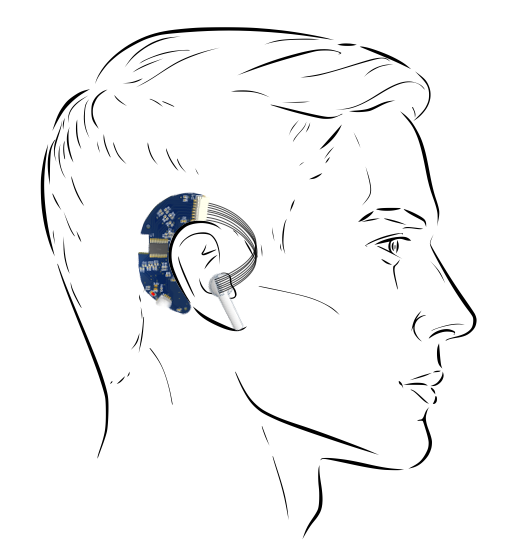
\includegraphics[width=0.48\textwidth]{thesis-doc/images/prototype/prototype_on_head_visual.png}
    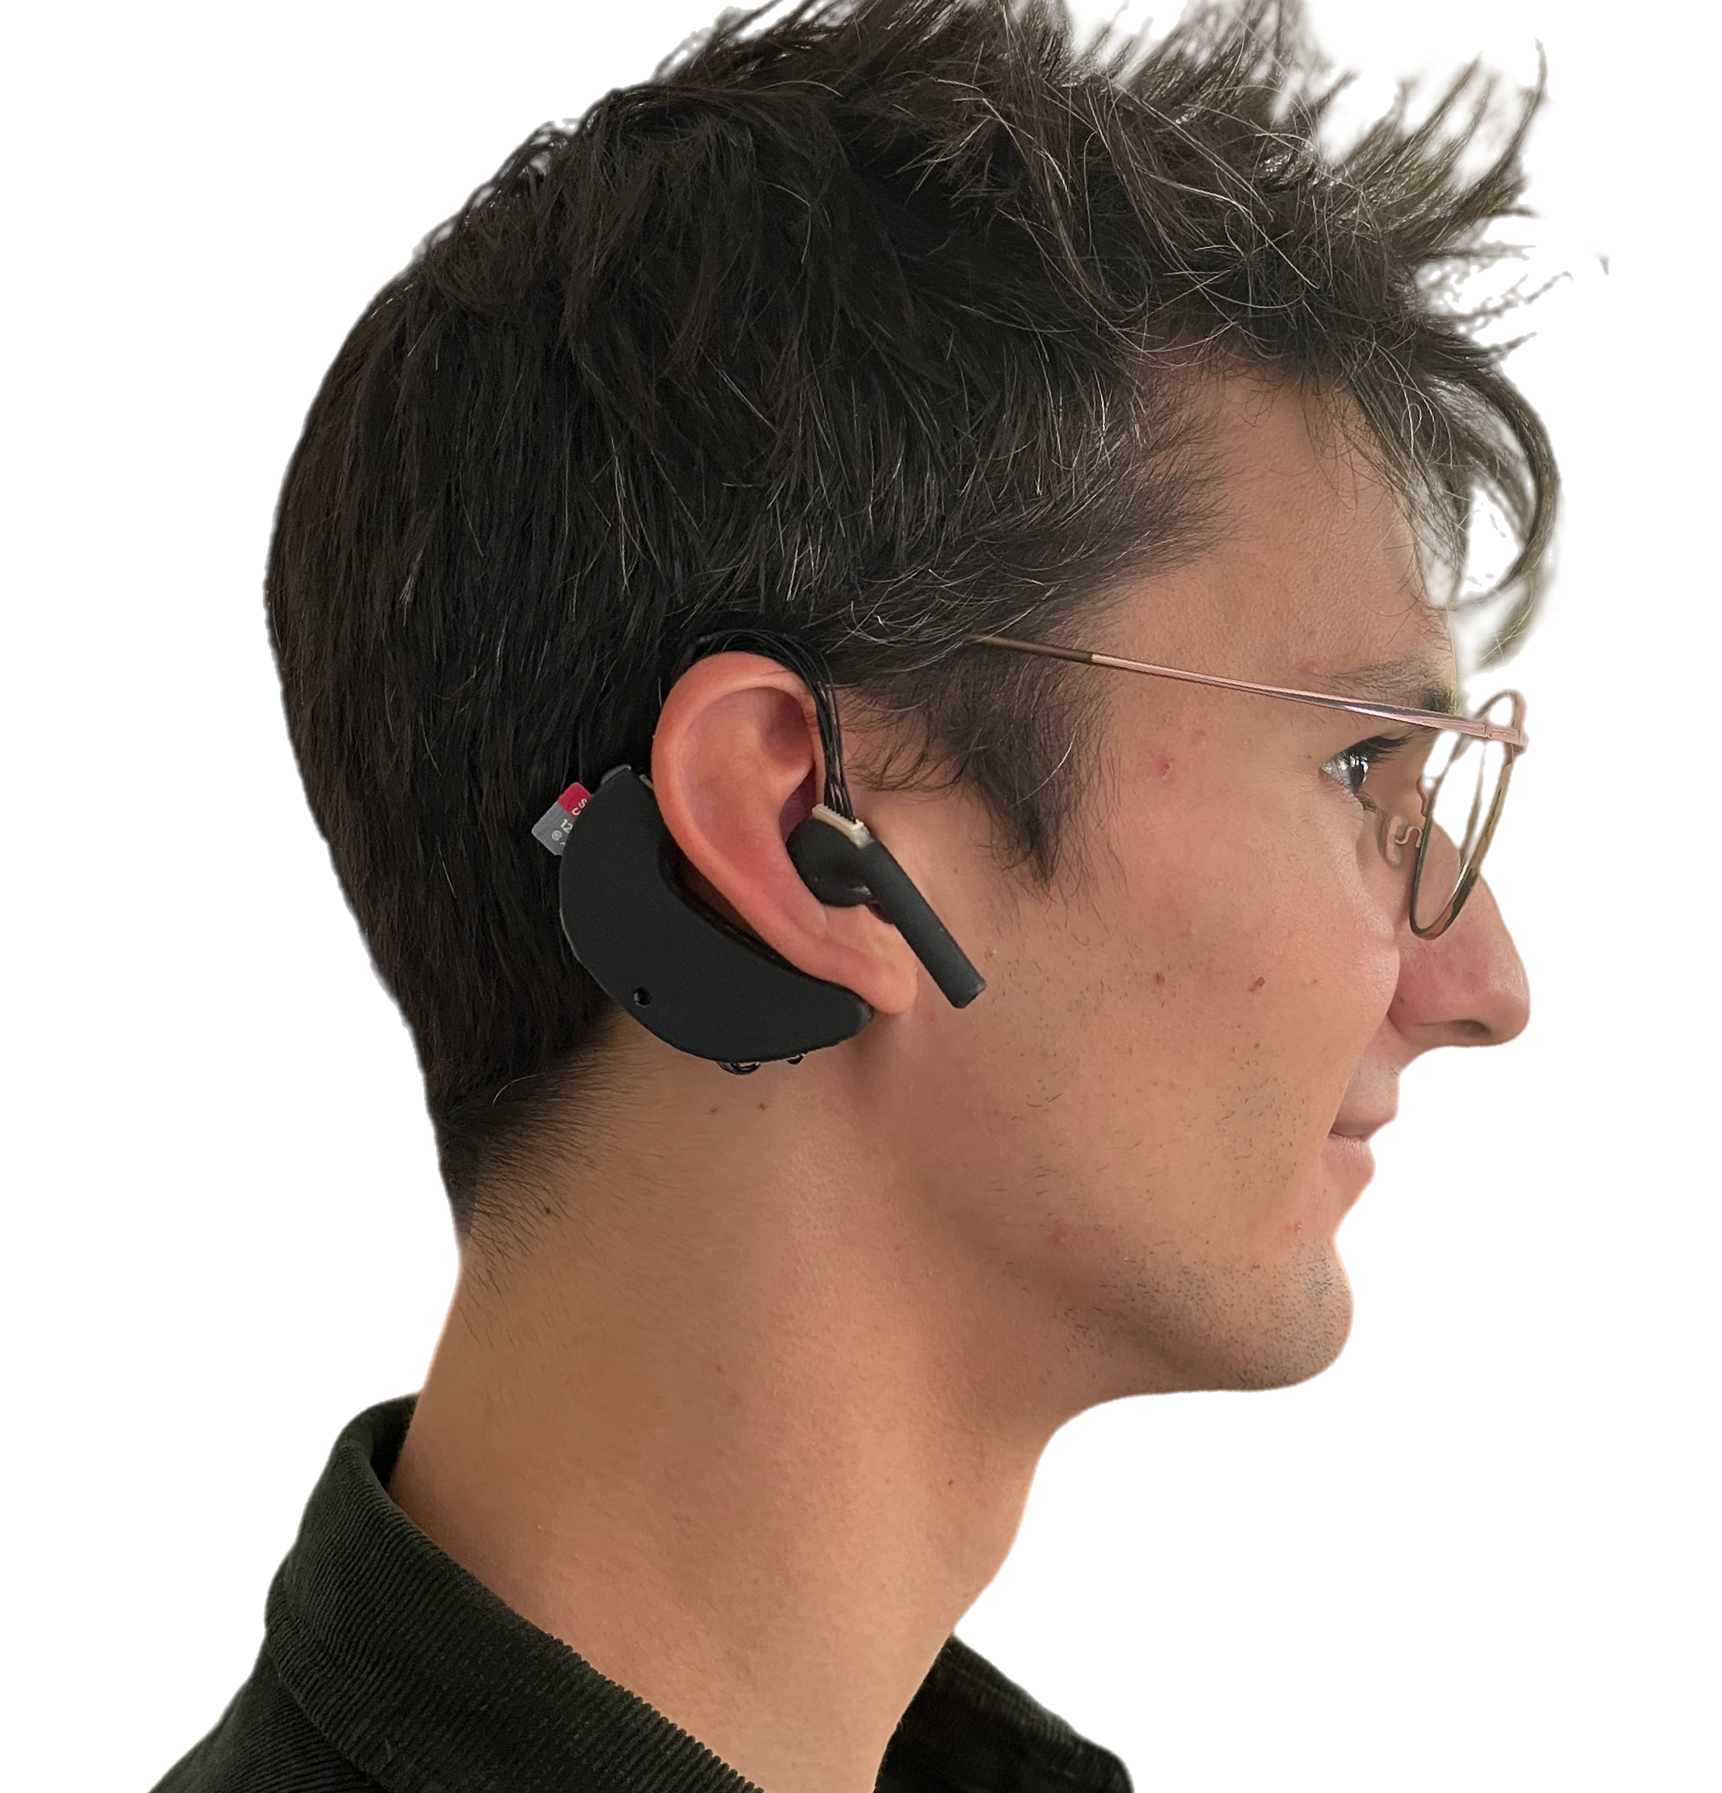
\includegraphics[width=0.48\textwidth]{thesis-doc/images/prototype/Lorenz.png}
    \caption{Visual view while wearing the components, next to it a real view. The PCB behind the ear measures in three positions (bottom, middle, top) and is connected to the FlexPCB via an 8-pin connector, which is visually already wrapped in the case here in the right picture. The wiring of the two components results in good stability when worn so that the device cannot fall off. In addition to this visual representation, the prototype can be viewed in a real environment including the cases.}
    \label{fig:design:prototype_on_head_visual}
\end{figure}

\begin{figure}
    \centering
    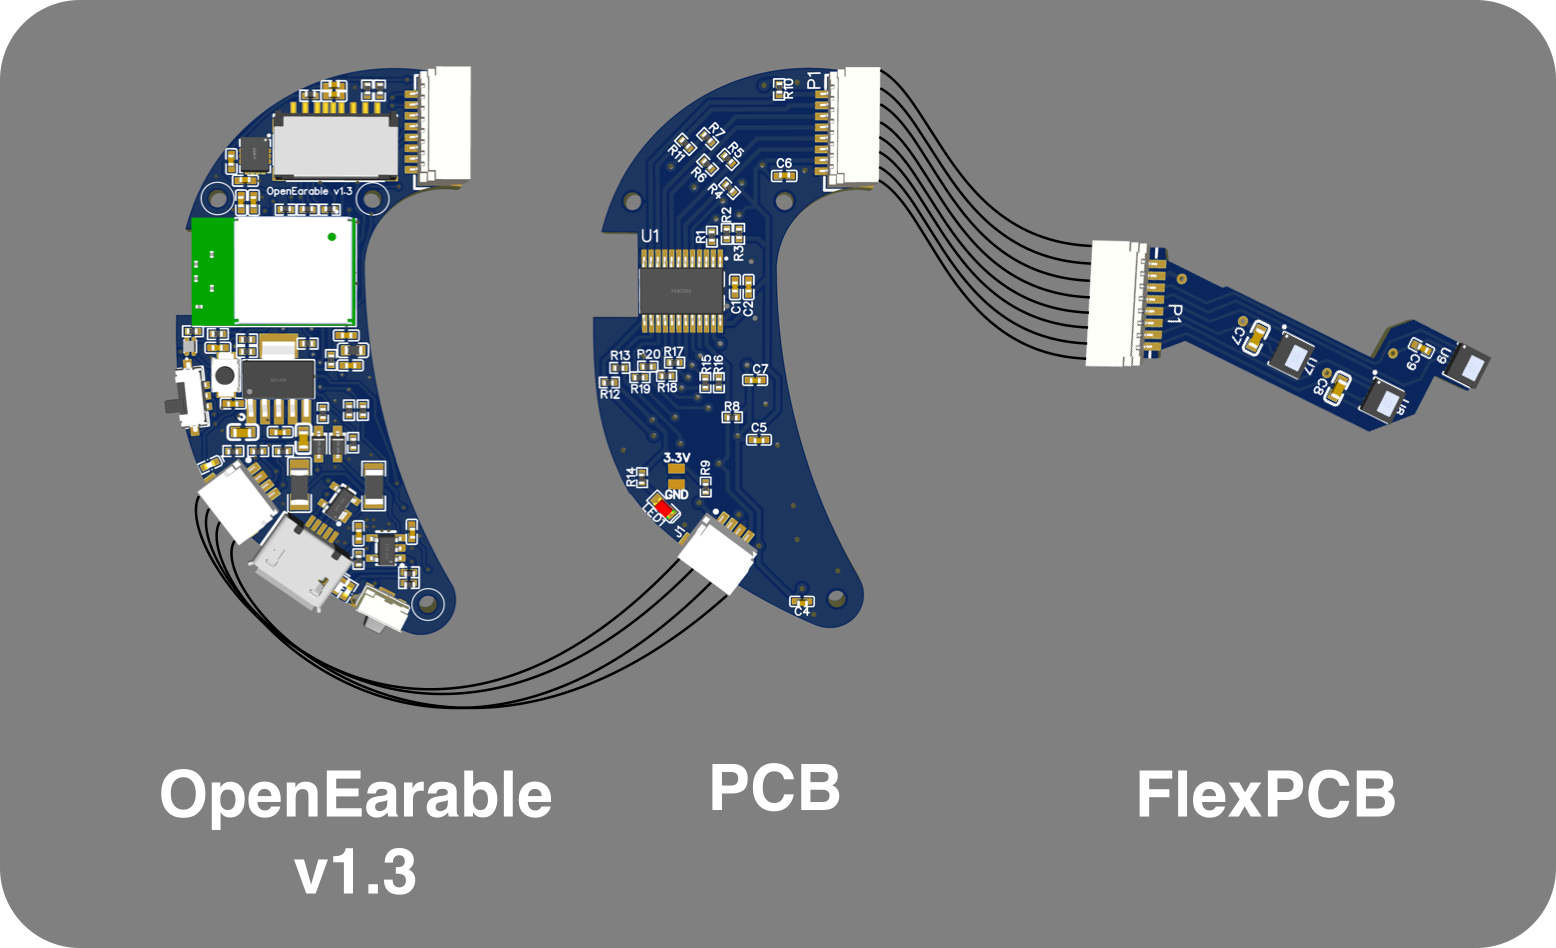
\includegraphics[width=\textwidth]{thesis-doc/images/prototype/PrototypeConnection.png}
    \caption{Visual representation of the prototype and the interaction of all components. The PCB is connected to the OpenEarable v1.3 with a 4-pin connector. In the OpenEarable is an Arduino Nano33 BLE, with which it is possible to control the multiplexer (TCA9548A) via I2C. Through this, every sensor value on the PCB and also on the FlexPCB can be read out, since the FlexPCB is also connected to the multiplexer via the 8-pin connector.}
    \label{fig:design:prototype_connection}
\end{figure}

\begin{figure}
    \centering
    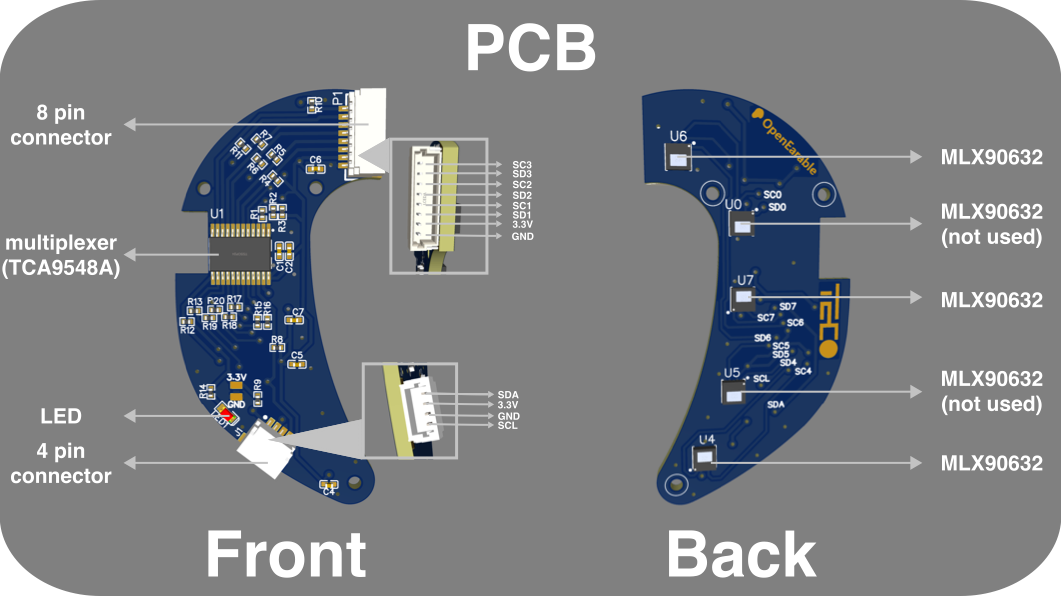
\includegraphics[width=\textwidth]{thesis-doc/images/prototype/PCB_Description.png}
    \caption{Representation of the front and back of the PCB. The multiplexer can be seen on the front, which is controlled by the OpenEarable via the 4-pin connector. The three other MLX90632 are then connected by the FlexPCB via the 8-pin connector. In addition, an LED is connected to the front, which lights up green if no short circuit is generated. The temperature sensors can be seen on the back, but only three of the five connections visible in the design are used.}
    \label{fig:design:pcb_description}
\end{figure}

\subsection{Temperature Measurements Behind the Ear}
\label{ch:Design:Prototype:BehindEar}

The temperature behind the ear is measured at three positions, as can be seen in Figure \ref{fig:design:pcb_description} on the back of the PCB and conceptually in Figure \ref{fig:ear_measurement_positions}.
To position the temperature sensors at the locations chosen in section \ref{ch:Introduction:PlannedApproach}, a PCB was developed that has the sensors installed at the appropriate locations. 
The PCB has been designed so that only the temperature sensors are placed on the back. This allows the PCB to be placed entirely in the bottom of the case, while the temperature sensors peek out through matching openings in the case. On the front of the PCB are all the other components, including a 4-pin connector and an 8-pin connector.
The 4-pin connector is used to connect to the OpenEarable. This connection allows the OpenEarable to communicate with the PCB via I2C, as the OpenEarable also has a special 4-pin connector for this purpose.
To be able to control the second component (the earpiece) via I2C later on as well, the 8-pin connector was added to establish a connection to the second component.
Via I2C, the built-in multiplexer is addressed, with which one of the eight possible applied lines can be switched and read out. The eight possible through-connections of the multiplexer are connected to all temperature sensors, including those of the FlexPCB via the 8-pin connector.
In addition, an LED is installed on the PCB to directly indicate a possible short circuit.
For each temperature sensor, the signals Ground, Power (3.3V) as well as SCL (clock signal) and SDA (data transmission) are required, as shown in Figure \ref{fig:design:pcb_description}. Communication with the multiplexer can be handled through the 4-pin connector.
To connect the three temperature sensors of the FlexPCB, a total of 12 signals are required, which can be reduced somewhat. For this purpose, the ground and power signals can be used together, resulting in a total of 8 signals being transmitted.

A case has now been developed around the OpenEarable and the custom-made PCB to enable a comfortable fit.
Above the PCB, the battery is placed in the enclosure so that no long cables are needed for the power supply to record the data in the study conducted.
The OpenEarable is placed above this.
The dimensions of the PCB are exactly the same as the OpenEarable to keep the case as small and compact as possible.
The sensor used requires an angle of $ 50 ^ \circ$ around itself for the temperature to be reliably measured. 
This was taken into account.
% The layered representation for visualization can be seen in Figure \ref{fig:design:prototype_behind_head_layered_view}.

% \begin{figure}
%     \centering
%     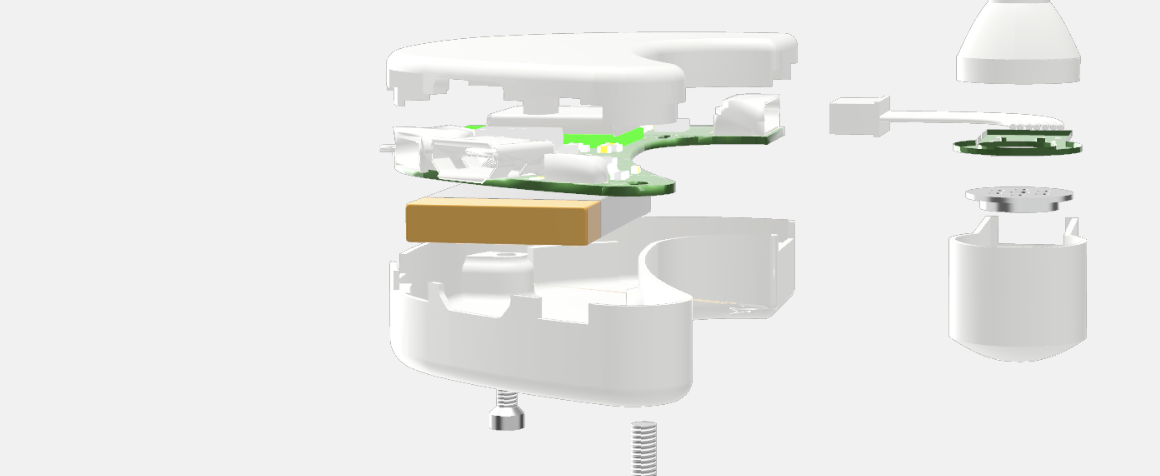
\includegraphics[width=\textwidth]{thesis-doc/images/prototype/Prototype_PCB_layered_view.png}
%     \caption{Layered view of the component behind the ear. At the bottom is the designed PCB as the temperature sensors can look out towards the skin. The battery is placed between the PCB and the OpenEarable.}
%     \label{fig:design:prototype_behind_head_layered_view}
% \end{figure}

\subsection{Temperature Measurements in the Ear}
\label{ch:Design:Prototype:Earpiece}

The second component now enables temperature measurement in the ear area. The FlexPCB itself is only equipped with components on the front side. Thereby, the 8-pin connector that connects the FlexPCB to the PCB is located, as described in section \ref{ch:Design:Prototype:BehindEar}.
Additionally, three temperature sensors are placed on the FlexPCB to sense the positions in the ear and pinna described in section \ref{ch:Introduction:PlannedApproach} and Figure \ref{fig:ear_measurement_positions}.
The FlexPCB was designed to extend through the component. On the one hand, the 8-pin connector protrudes outward to connect to the PCB. 
On the other hand, the PCB runs along the outside of the housing to the earbud, allowing the FlexPCB to snake through. 
The tip of the FlexPCB also contains a temperature sensor mounted in the earplug and aimed directly at the eardrum. 
Another temperature sensor is aimed at the ear canal and is located on the outer edge of the earplug. The third temperature sensor is aimed at the pinna.
The component was modeled on the design of an AirPod, but heavily modified afterward. 
The original AirPods design is freely available on TinkerCAD and was used as the basis for the component shape. 
The inside of the design was completely hollowed out to allow cables to be routed through the case. Additionally, an adapter was added to the side to fit the redesigned earpod. 
An earbud can be attached here to ensure that the earbud penetrates further into the ear than usual compared to conventional in-ear headphones. 
This enables precise temperature measurement in the direction of the eardrum. A temperature sensor is attached to the tip of the earbud to perform basic temperature measurements.
The three temperature sensors on the FlexPCB can be switched via the multiplexer that is connected to the PCB. 
This allows for precise selection and acquisition of the desired measurements. Figure \ref{fig:design:prototype_earpiece_views} shows a sketch and other images of the final component.

\begin{figure}[!h]
    \centering
    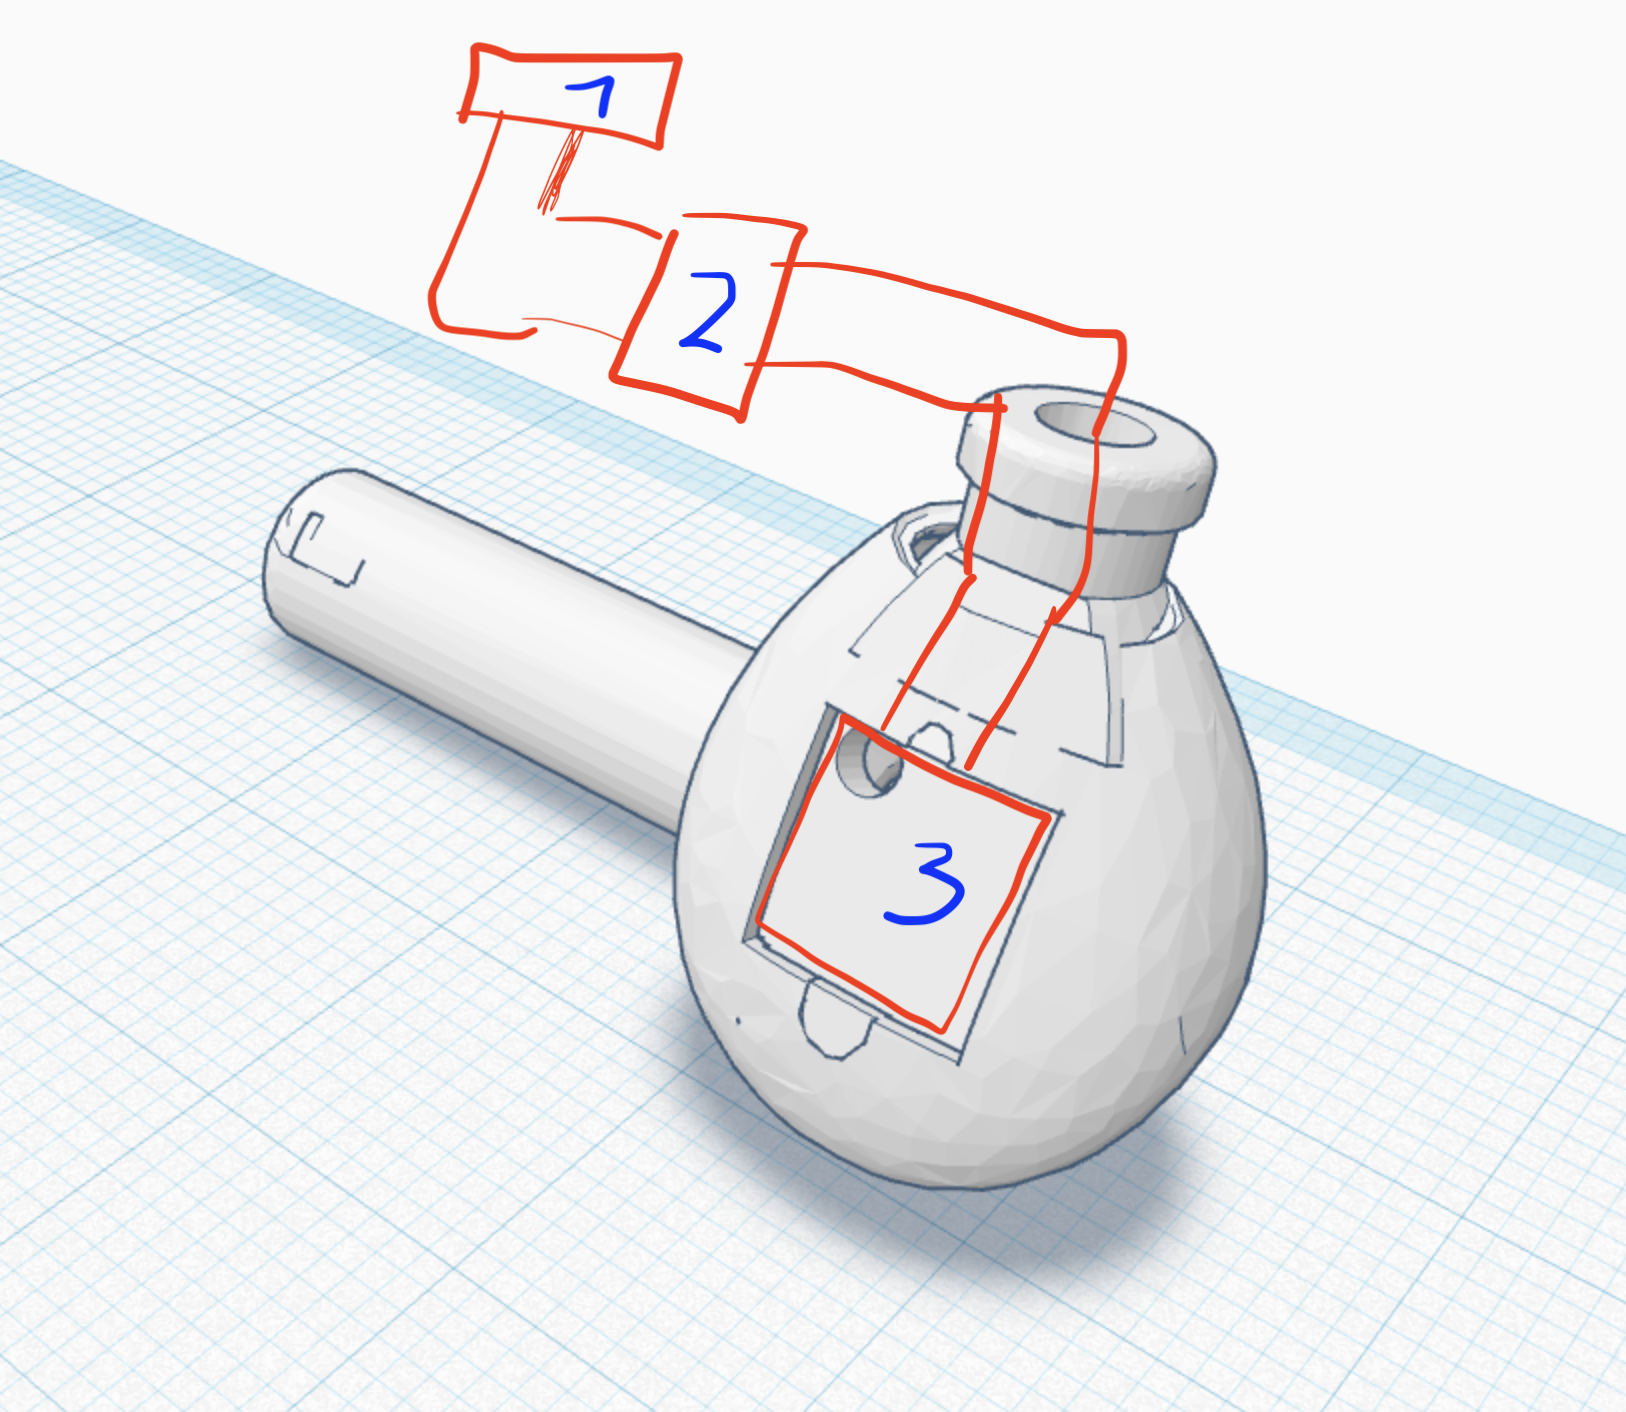
\includegraphics[width=0.48\textwidth]{thesis-doc/images/prototype/flex_pcb_design_finding.png}
    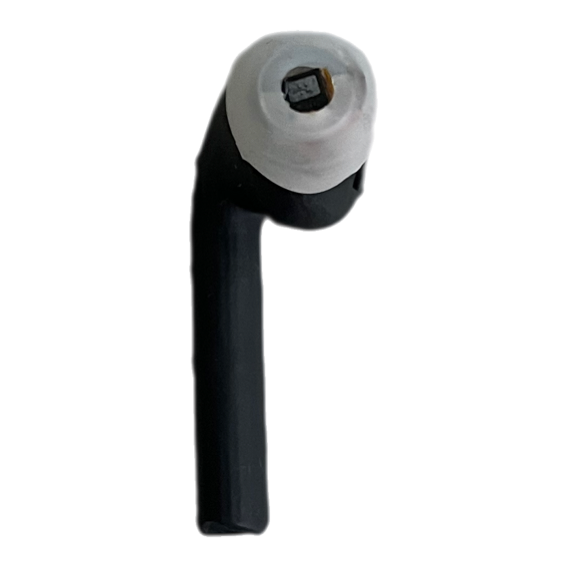
\includegraphics[width=0.48\textwidth]{thesis-doc/images/prototype/Earpod_Front.png}
    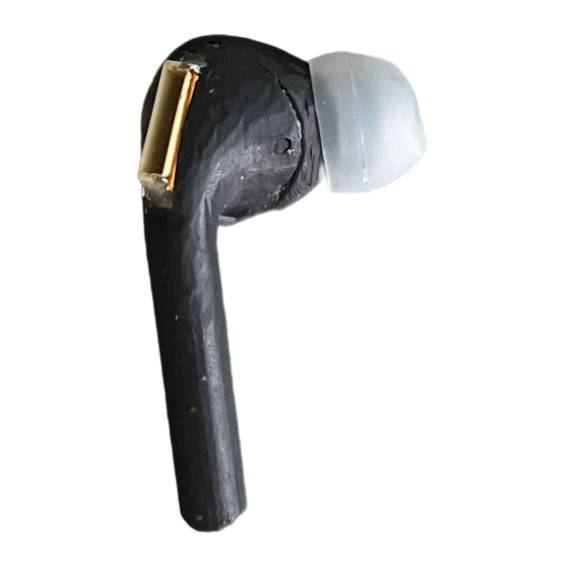
\includegraphics[width=0.48\textwidth]{thesis-doc/images/prototype/Earpod_Side1.png}
    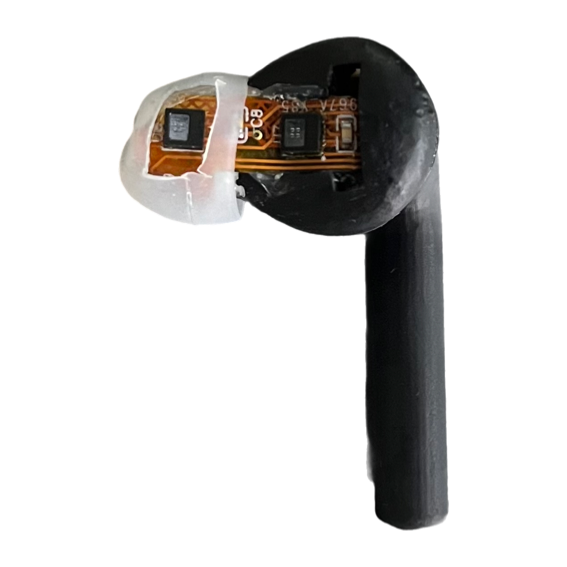
\includegraphics[width=0.48\textwidth]{thesis-doc/images/prototype/Earpod_Side2.png}
    \caption{Sketch and real view of the earpiece from different perspectives.
The sketch shows the first idea of how the FlexPCB has to be designed so that it gets through the earplug to the tip to measure in the direction of the tympanic membrane. The real views provide an impression of how the component is composed. On the bottom right picture, you can see the sensors on the concha and ear canal, on the top right picture the sensor directing to the tympanic membrane. The bottom left picture displays the 8-pin connector.}
    \label{fig:design:prototype_earpiece_views}
\end{figure}

\section{Study}
\label{ch:Design:Study}
The requirement of this master thesis is to measure the temperature at different positions of the ear to enable temperature measurement over a longer period of time. 
For this purpose, a study is to be conducted in which the temperature is measured at different positions and then compared. 
For this purpose, a prototype was developed, which was described in detail in the previous chapters. 
With this prototype, it is possible to measure the temperature at three positions behind the ear, on the auricle, in the ear canal and on the eardrum.
The goal after recording the data is to compare the different positions. 
In the context of this master's thesis and related study, several hypotheses arise that have the potential to clarify key aspects of ear temperature measurement. 
One of these hypotheses concerns location-dependent temperature accuracy. It is hypothesized that the position of the sensors, whether behind the ear, in the pinna, in the ear canal, or on the eardrum, significantly affects the accuracy of the temperature measurement.
Furthermore, the question of replicability and consistency of the measurements is of interest. It is assumed that despite the variable human physiology, the measurement results are consistent across different subjects. The relevance of the initial acclimatization phase of the sensors is also considered. Here, it is assumed that the 20-minute acclimatization phase is sufficient to ensure stable temperature measurement. 
The role of environmental variables is also considered. 
It is hypothesized that the readings could differ significantly from the baseline measurements after being outdoors, allowing conclusions to be drawn about the susceptibility of the sensors to environmental conditions. 
In addition, the adaptability of the measurements to changing temperature conditions is another key issue. 
It is hypothesized that the sensors will respond quickly enough to detect and account for changes in ambient temperature while outdoors.
In the context of the further hypotheses, for example, the question is raised whether changes in the IMU signal, i.e. in the gyroscope, magnetometer and accelerometer measurements, are correlated with changes in temperature. Similarly, the relevance of the physiological nature of the subjects, such as the skin thickness behind the ear or the ear shape, is highlighted in relation to the measurement accuracy. 
Finally, the speed of the sensors in detecting rapid temperature changes induced by physical or emotional states is considered as a possible variable for assessing system performance.
These hypotheses not only provide a broad basis for evaluating the developed prototype, but can also be used to define further research questions and applications in the field of temperature measurement by wearables.
% Write more about stress study

\subsection{Study 1: Localized Ear Temperature Measurement Study Procedure: Baseline Surveys and Environmental Influences}
\label{ch:Design:Study:Study1}
Two studies were conducted as part of this master's thesis. 
The first study deals with the comparison of the temperatures at the different positions.
For this purpose, a study was designed to test the different hyptotheses and to create the best possible data basis. 
The study starts with the temperature measurement of the right ear by a thermometer (BRAUN ThermoScan 7) to obtain a reference value of the temperature in the ear. 
This measurement will be taken again at the conclusion of the study.
This is followed by the attachment of the prototype to the subject's ear. This phase is critical, as correct positioning of the sensors is crucial for the quality of the recorded data.
Since the component behind the ear tends to stick out a bit from the skin after a while, the component was taped behind the ear to be securely in the correct position and not slip even during light activities. 
A powerbank was attached to ensure that the prototype's battery lasts for the complete period, as initial findings indicate that the battery life is between one and two hours.
After the installation of the prototype, an acclimatization phase of 20 minutes follows, during which data is already recorded. 
This phase is to ensure that the sensors have sufficient time to adapt to the physiological conditions of the subject and to allow stable measurements.
After completion of the acclimatization phase, the main data collection is performed. 
The subject spends another 20 minutes in a seated position in a room of the institute where all other subjects have also performed the study. 
The room is not air-conditioned and the windows were closed before the measurement.
In addition, the room temperature and humidity were noted. 
This phase is to provide a baseline for the temperature measurements and to verify the consistency of the sensors under stable conditions.
The next step is to investigate the influence of environmental variables. 
Subjects will be asked to spend time outdoors walking for 20 minutes. 
This is done to analyze the response of the sensors to sudden changes in temperature and environment and to evaluate the adaptability of the system.
After returning indoors, subjects again sit in their original seats and remain in a seated position for another 20 minutes. 
This phase allowed for quantification and analysis of any deviations in sensor measurements due to being outdoors.
Throughout the time in the room, subjects were allowed to watch animal documentaries that allowed for no or minimal anxiety or happiness. 
In total, the study will be conducted with 15 subjects to provide a sufficient database for statistical analyses.
A visual diagram of the procedure during study 1 can be seen in Figure \ref{fig:design:study1:procedure}.

\begin{figure}[t]
    \centering
    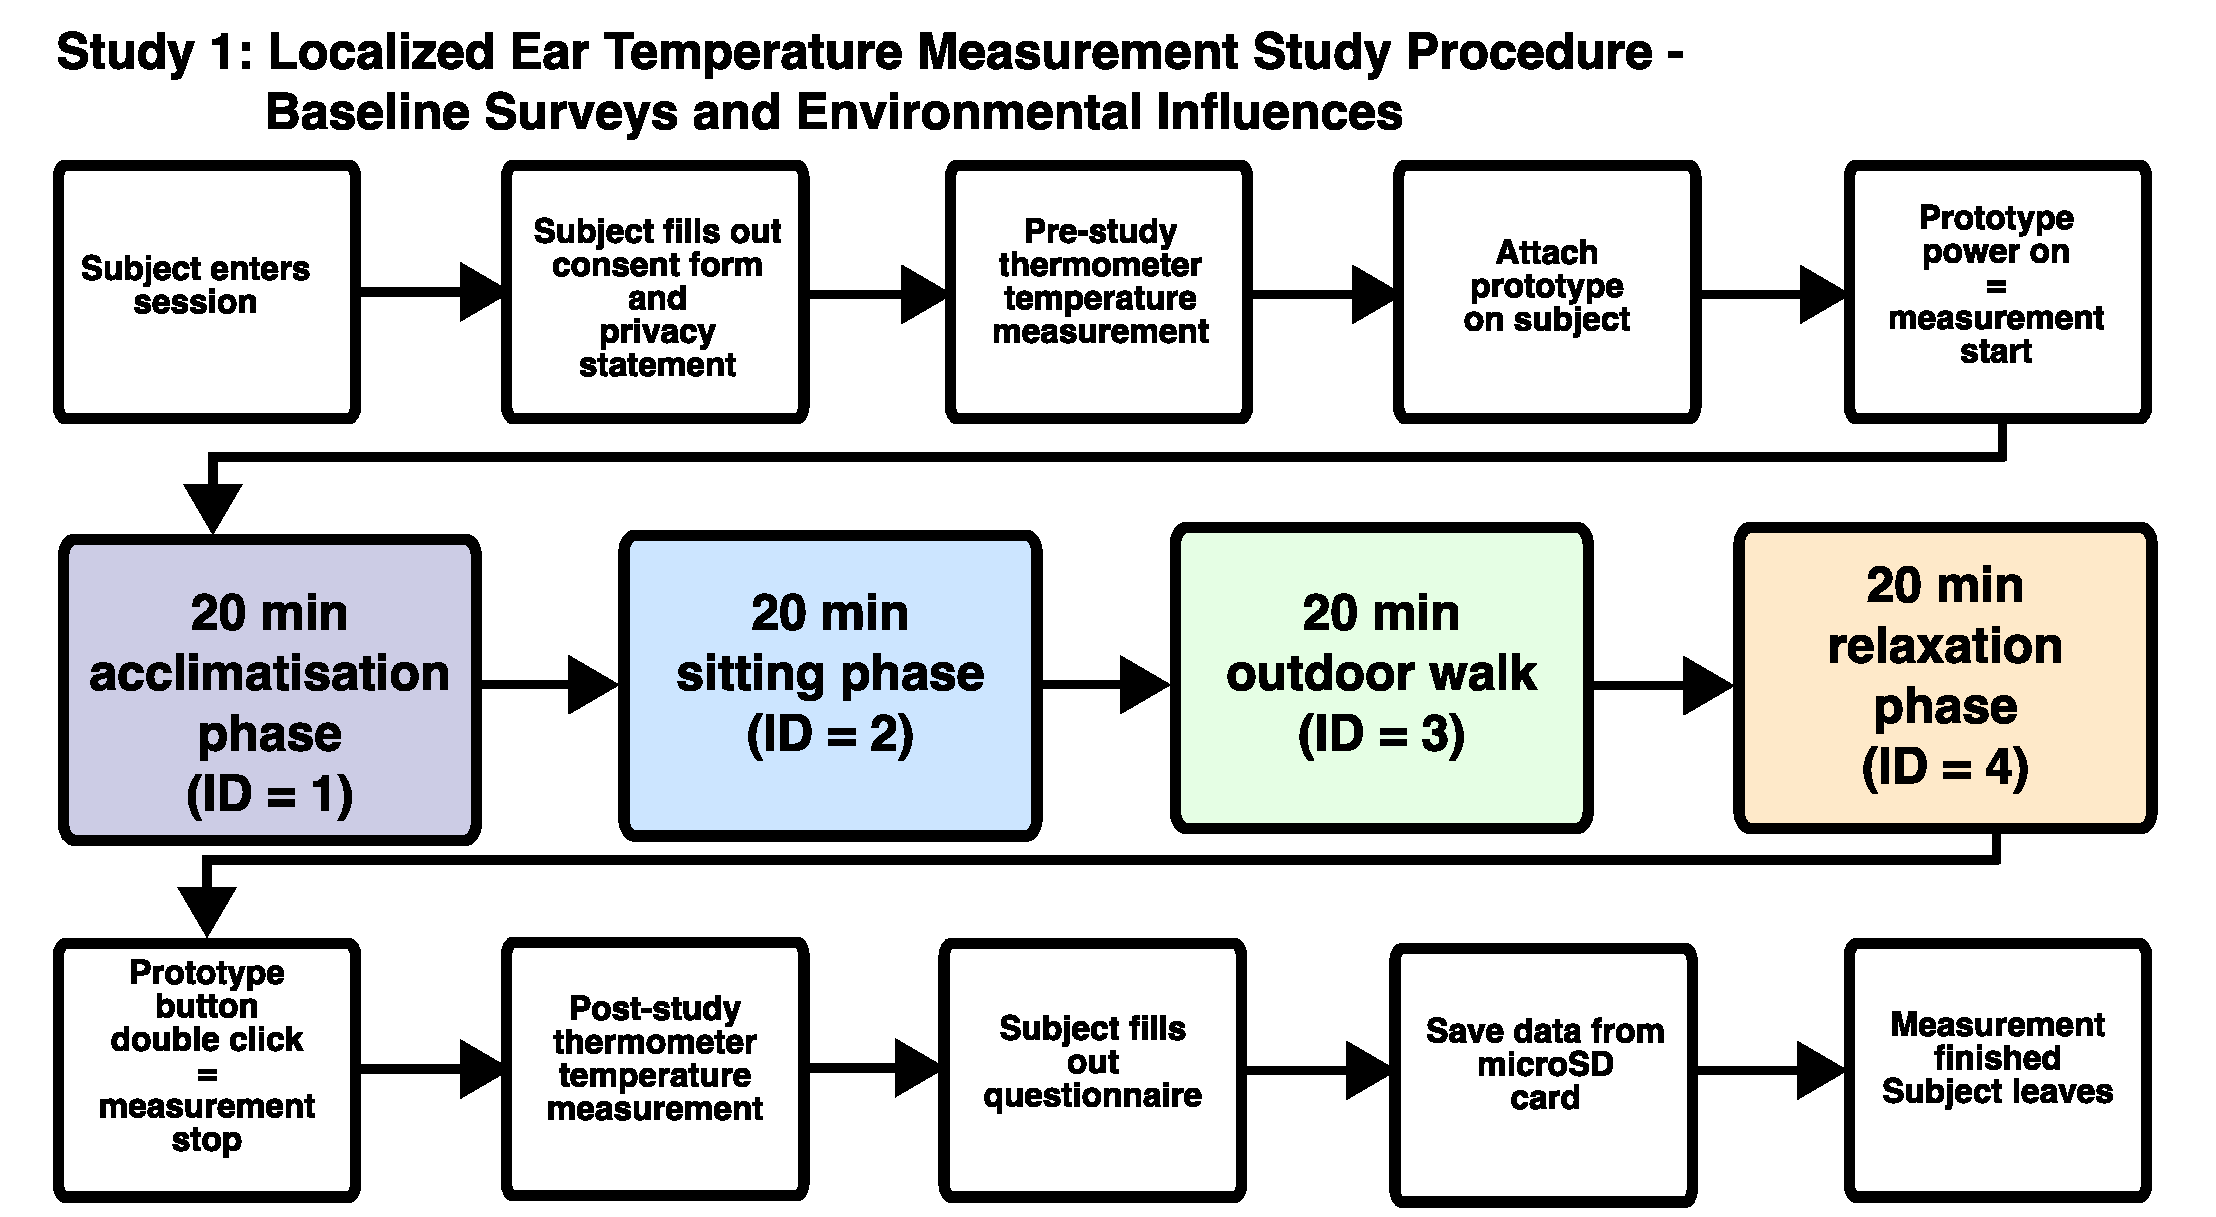
\includegraphics[width=\textwidth]{thesis-doc/images/study1/Procedure.pdf}
    \caption{ADD DESCRIPTION}
    \label{fig:design:study1:procedure}
\end{figure}

Through this carefully designed procedure, the study is expected to help test the formulated hypotheses and provide valuable insight into the performance of the developed prototype and its potential applications.

\subsection{Study 2: Study Course Under Stress Conditions: Impact on Temperature Measurements With Ear-Based Sensors}
\label{ch:Design:Study:Study2}
In the second study, the influence of stress-induced physiological changes on temperature measurements at different sites of the ear is investigated. 
An initial 20-minute acclimatization period, during which the sensors and the subjects adapt to the environmental conditions, is followed by a 15-minute measurement period in a seated position.
After that, the subjects are exposed to a stress situation. 
At the beginning of the stress phase, the subjects solve a Stroop test, then an N-Back test and finally a mathematics test. 
The Stroop test tests the subjects' attention by alternately displaying words in different colors. 
The subject is asked to interpret the color of the word. The words are always color words, but the words do not always match the color in which they are displayed. 
When the word and the color do not match, the reaction time and the number of errors increase. 
This is to create an initial stress situation for the subject \cite{StroopCompetitionSocialEvaluative}. 
Next, an N-back test with 2 dimensions is performed. 
Here, a letter is named to the subject via a voice output and a position in a tic-tac-toe field is displayed. 
The subject must now recall N steps back and indicate whether the letter or position has already been named or shown in the last N iterations. 
This test was performed with $N={1,2,3}$ and is designed to elicit strain and stress \cite{liangEffectAcuteStress2023}.
Last, the subject is presented with a mathematical test. 
This involves several mathematical tasks in which 4 answer options are always available.
Here, the subject has 8 minutes to solve as many tasks as possible. 
This is also designed to trigger a stress situation \cite{caviolaStressTimePressure2017}.
The three tests are all designed to trigger stressful situations and always challenge the subject in a different way.
For the Stroop test, there is no visual timer, but the number of words is limited. 
There is a high score for the test, which is intended to motivate the subject to do as well as possible. 
In the N-Back test, the time is strictly given, the subject has the opportunity to answer within three seconds.
Here, the subject is exposed to the risk of being frustrated if he or she fails to complete one or more sub-steps.
The mathematical test has a time limit of 8 minutes, in which the subject must solve as many tasks as possible.
Again, the subject is put under pressure in a different way that is intended to trigger stressful situations.
This scenario was chosen because a large study was not possible due to time constraints. 
Standard in science for induction in standardized stress induction tests is the Trier Social Stress Test (TSST). 
However, the selected test covers the requirements and should allow to induce stress in the subjects.
To check the stress level of the subjects, heart rate is measured in addition to temperature data. 
These additional markers provide a solid scientific basis for evaluating stress induction and its effects on the measured temperature values.
The stress induction phase is followed by another 15-minute measurement phase in a seated position, during which the subjects are not exposed to any other stressful situations. 
This serves to record the recovery processes and their effects on the measured parameters. 
In study 2, the effect of different stress-inducing tests - the Stroop test, the N-back test and a timed mathematical test - on the temperature measurement at the ear is investigated.
At the same time, heart rate will be measured as an additional physiological marker of stress. 
The study includes an initial acclimation phase, a pre-stress measurement phase, a stress induction phase and a post-stress measurement phase to comprehensively assess ear temperature variations under stress conditions.     % Entwurf
\chapter{Implementation}
\label{ch:Implementation}
This chapter describes the details of the implementation of the prototype and the analysis of the data collected during the studies.
To implement the prototype, Arduino software was developed to measure temperature sensor values and IMU data and store them on a microSD card with a timestamp.
Implementation details for evaluating and analyzing the collected data are described afterwards.

\section{Prototype}
The prototype is controlled by OpenEarable, which was programmed to be controlled via Arduino code. 
An Arduino Nano33 BLE is built into the OpenEarable, which facilitates customization. 
The main task of the prototype is to collect data from the temperature sensors and an IMU and store it in a CSV file on the SD card, which has its own slot in the OpenEarable. 
Similar to traditional Arduino code, the prototype code consists of a \texttt{setup()} and a \texttt{loop()} method.

In the \texttt{setup()} method, all the required components are initialized. These include the sensors, the IMU, the SD card logger and the key interrupt. The latter is used to ensure that a measurement is terminated should the key be pressed twice within two seconds. If the key is pressed once, the phase is changed (ID). 
When the sensors are initialized, a \texttt{Wire} connection is made and the multiplexer is triggered.
The multiplexer is crucial when reading out the sensors, because each sensor is addressed with the same address.
All temperature sensors are connected to the multiplexer and are addressed one after the other to read out the temperature value.
This is possible because the multiplexer always switches through one output and thus all sensors can have the same address.

In addition to the regular operations in the \texttt{loop()} method, the code contains functions for handling keystrokes. A key press is detected using an interrupt. As soon as the key is pressed, a function is started that checks whether the key has already been pressed within the last two seconds. If this is the case, the data acquisition of sensor data and IMU data is stopped and the SD card with the collected data is written.

One of the main tasks is to read data from the MLX90632 sensors and the IMU sensor. 
For this, the multiplexer is always switched to the respective sensor and the value is read and persisted via the modified library "Protocentral\_MLX90632".
The library was strongly modified to enable a faster measurement. 
This is necessary because additional motion data should be recorded.
The IMU sensor, built directly into the OpenEarable, provides accelerometer, gyroscope and magnetometer data.

The collected data from one pass of the \texttt{loop()} function is then written to the SD card. Each line represents one pass of the \texttt{loop()} function and contains one of the 6 temperature sensor values and the 9 IMU data as well as a time value and an ID.
Thus the 6 temperature sensor values are distributed in 6 lines. 

Furthermore the library "Protocentral\_MLX90632" was adapted. In the original library, the \texttt{getObjectTemp()} function waits for the temperature value to become available by waiting in a \texttt{while} loop for a register value to be set indicating newly available data. This resulted in an unacceptably long wait time because the update rate per sensor is 2 Hz. 
During this time, no IMU data signal can be read due to the \texttt{while} loop present in the library, as the Arduino Nano33 BLE does not allow parallelism. 
To fix this problem, the check to see if new data is available is ignored. 
Instead, the temperature value is read in each loop iteration. 
As a result, the temperature value may not have updated yet. 
However, the sampling rate is so high that this does not affect the final result.
The IMU data needs a sampling rate of at least 50Hz to make significant statements about the motion. 
To achieve this, only one sensor value per iteration was read out to achieve the performance. 
Additionally, the code had to be optimized several times for performance reasons, ranging from removing \texttt{for} loops to storing data in strings, instead of arrays. 
Finally, a sampling rate of $50Hz$ of IMU data and a sampling rate of $8.3Hz$ of sensor values has now been achieved.
Since the temperature sensors have an update rate of $2Hz$, some consecutive sensor values are the same, but no measured sensor value is lost.

\section{Sensor Calibration Implementation in Arduino}
The calibration was implemented using the Arduino platform, modifying the library for the MLX90632 sensors to introduce an emission factor of $0.98$ according to the sensor datasheet. 
This value is optimized for measuring human body temperature and was also used for the metal plate during calibration. 
This emission factor allows the system to account for the natural variability of thermal radiation between different materials and provide a standardized reading that is consistent across environments.

\section{Data Analysis with Python}
A pipeline was created for each of the analyses of Study 1 and Study 2. 
The pipeline first reads all the recorded data into a Pandas data frame and generates the results for the different hypotheses.
For each hypothesis, a file exists: "hypothesisX.py", where the "X" stands for the number of the hypothesis. 
This is called in the pipeline and all results are either output or the plots are saved in the "target" folder.

In the analysis of Study 1, Python's Pandas library is used to import the raw data collected from the sensors. 
The reference thermometer value collected by the BRAUN ThermoScan 7 is also stored per subject. 
Any erroneous or missing data points are identified and either removed or interpolated to maintain data quality. 
Since only one temperature sensor value is stored per measurement and the other 5 sensor values are set to 0, they are also set to "NaN", which greatly simplifies the subsequent recording of the data.
During the acclimatization phase, the data is not evaluated, since this phase serves to acclimatize the sensors to the temperature and leads to constant measured values.
In addition, the "ID" represents the separation of the phases.
In order to compare different temperature readings between multiple individuals, the ground truth, i.e. the thermometer reading, is subtracted from each sensor reading.
The individual hypotheses are now analyzed and further supported by a significance test (paired t-tests) to prove or disprove the hypotheses.
Visualization tools from the Matplotlib and Seaborn libraries will be used to visually represent temperature variations, sensor stability and the effects of environmental variables.
In the second study, raw data will be imported and temporally aligned similar to study 1. Heart rate data will also be imported and synchronized with temperature measurements. 
Data quality is checked to ensure the integrity of the data set.
For data analysis, temperature changes during stress induction tests, which include the Stroop test, N-back test and math test, will be examined. 
Inter-subject variability and consistency will also be assessed. 
Heart rate data will be used as baseline data for stress induction. 
Significance tests (t-tests) will also be used to evaluate the effects of stress on temperature measurements. 
Correlations between changes in heart rate and temperature will be analyzed to provide evidence of the effects of stress induction. 

In both Study 1 and Study 2, custom Python pipelines were developed to process and analyze sensor data, using Pandas for data manipulation and Matplotlib and Seaborn for visualization. These pipelines read raw sensor and reference thermometer data into Pandas data frames, performed quality checks and performed hypothesis-specific analyses. The resulting statistical or visual insights were then stored for further analysis. Study 1 focused on sensor stability, temperature fluctuations and environmental effects, while Study 2 expanded the analysis to include stress-induced effects and heart rate correlates.    % Implementierung
%% eval.tex
%% $Id: eval.tex 5 2005-10-10 20:55:48Z bless $

%%%%%%%%%%%%%
\chapter{Evaluation}
\label{ch:Evaluation}
%%%%%%%%%%%%%
        % Evaluierung
\chapter{Conclusion and Future Work}
\label{ch:Conclusion}

\section{Conclusion}
In this master's thesis, the field of ear-based temperature sensing was studied in depth, with a focus on sensor placement and evaluation for wearable applications. 

The research began with the design and development of a prototype equipped with temperature sensors at various locations on the ear. 
The development of this prototype was a critical step because it enabled the collection of temperature data with high accuracy, which served as the basis for subsequent analysis. 
The prototype demonstrated the feasibility of ear-based temperature monitoring and its potential applications in healthcare and beyond.

The initial study, which focused on local temperature measurement at the ear, provided valuable insight into the intricacies of ear-based temperature sensing. 
It highlighted that sensors require an acclimation period to adapt to individual physiological conditions. 
It was also clearly seen that the temperature sensors always took different lengths of time to adapt to the new conditions.
In addition, the study confirmed the reliability and stability of temperature readings at different locations on the ear. 
The results showed that the sensors were quite stable after the acclimation period, confirming the usefulness of the prototype for long-term temperature monitoring.
While people sit in a room, the temperature of each sensor hardly changes, but it is constantly different between sensors.
This is due to the different positions, as each has different temperatures.
While the subjects went outside for a walk after the 20 minute sitting period, there was a noticeable drop in temperatures. 
The further the sensor was in the ear, the less the temperature changed.
Here, it was clearly seen that the sensors were exposed to external conditions, such as the temperature drop (approximately $5^\circ\text{C}$ outdoor temperature), wind, sunlight, and other conditions.
After the subjects arrived back in the room, the temperature settled back to the value measured earlier in the second phase.
In general, it was also shown that the variance in the outdoor phase was significantly higher than in the indoor phase (Phase 2).
In addition, the sensors behind the ear were shown to have lower temperatures than the sensors in the ear and at the concha.
Since motion data was recorded in addition to temperature, it was shown that the subjects exhibited increased relative absolute changes in the different temperature measurement points during the outdoor phase.
The most stable measurement was obtained with the sensor pointing to the tympanic membrane. 
Here, the measurement was very close to the ground truth and had the least environmental effects to show.

The second study focused on investigating the effects of stress on ear temperature. 
The study was designed with three different stress-inducing tests to provide a holistic view of the effects of stress. 
Due to limited capacity, a Trier social stress test (TSST) was not used, which is currently considered the best scientific option to induce stress.
In the study, five subjects were used for recording, in which initial tendencies were shown.
Only one subject had clear rashes of stress during the stress phase, the other subjects showed mild to no signs of stress.
It was recognizable that slight to strong signs were seen in male subjects and no signs of stress in female subjects.
However, this cannot be generalized directly because the number of subjects was too small (5, 3 male, 2 female).
When looking at temperature, no significant temperature increases were detected during stressful periods.
However, this is also not an indication that the temperature does not increase during stress, since on the one hand the number of subjects was much too small for this and on the other hand the optimal stress test was not selected due to time constraints.
Further studies are needed to provide clarity here.

Overall, the results of this research have implications not only for stress detection, but also for a broader range of applications such as health monitoring and potentially early disease detection.
The thesis successfully bridged the gap between theoretical concepts and practical implementation and provides a foundation for future work in this promising area.

\section{Future Work}
This chapter presents possible future work that can be built upon the foundation of this thesis.
This thesis focused on building a prototype, looking at its measured values in a first study and also collecting first findings on temperature changes under stress in a small scale.
Based on this, there are numerous areas which can be investigated with the new prototype.

\paragraph{Detection of Circadian Rhythm}
One of the most interesting avenues for future work is the study of circadian rhythm patterns through ear-based temperature measurements. 
By using the prototype, continuous temperature monitoring can provide data that can give insight into a person's biological clock and help diagnose and treat sleep disorders, among other things.
Here, across the different sensor positions, it is possible to test which sensor can be used to detect such patterns.
This could have far-reaching consequences should a sensor other than the sensor pointing to the tympanic membrane also detect such patterns. 
This is because it would then be possible to integrate such a sensor into a conventional in-ear headphone and monitor the body's temperature for a longer period of time.

\paragraph{Early Detection of Disease}
The prototype can also make a significant contribution to the detection of diseases, since, among other reactions of the body, the core body temperature also increases due to a defensive reaction to viruses and bacteria. Here, core body temperature is an early indicator of disease.
It could be checked whether this can also be detected by the various sensors of the prototype.

\paragraph{Cycle Tracking for Women}
Another promising application is tracking women's menstrual cycles. 
Body temperature is known to change slightly during the menstrual cycle.
Continuous monitoring via the ear could provide a non-intrusive method of tracking these changes. 
This could aid in fertility planning or in detecting irregularities that might require medical attention.

\paragraph{TSST for Stress Detection with Increased Sample Size}
To further validate stress detection skills, administration of the Trier Social Stress Test (TSST) could be beneficial in future studies. 
The TSST is a standardized procedure for inducing psychological stress and could provide a more comprehensive assessment of the prototype's stress detection abilities. 
This test would extend the second study conducted in this thesis.
This would again test the expected temperature increases, which were not detected in the setup used in this master thesis
Notably, the second study was conducted with a limited number of subjects. 
Future work could include a larger, more diverse population to statistically validate the results.

\paragraph{Real-World Applications}
Future work could include field studies in which participants perform everyday activities while wearing the device. 
This would test the robustness and applicability of the device in real-world conditions and potentially reveal unforeseen challenges or opportunities.
However, battery life would need to be optimized for this.
Activity classification would also need to be accurate.

\paragraph{Approaches to Machine Learning}
The rich dataset generated by the prototype could be used to train machine learning models for automatic detection of different physiological states or conditions to create a smarter, more adaptive system.

By pursuing these avenues for future research, this work can be expanded and refined and contribute to the growing body of knowledge in wearable health technologies.
The optimal position for detecting as many symptoms as possible, coupled with a position that fits into an everyday object such as in-ear headphones, provides tremendous scientific potential.
It also provides very important health values for the user, which he currently cannot obtain through any other alternatives.  % Future Work
\include{summary}   % Zusammenfassung und Ausblick

%% ++++++++++++++++++++++++++++++++++++++++++
%% Anhang
%% ++++++++++++++++++++++++++++++++++++++++++

\appendix
%\include{anhang_a}
%\include{anhang_b}

%% ++++++++++++++++++++++++++++++++++++++++++
%% Literatur
%% ++++++++++++++++++++++++++++++++++++++++++
%  mit dem Befehl \nocite werden auch nicht 
%  zitierte Referenzen abgedruckt
\cleardoublepage
\phantomsection
\addcontentsline{toc}{chapter}{\bibname}
%%
%\nocite{*} % nur angeben, wenn auch nicht im Text zitierte Quellen 
           % erscheinen sollen
%\bibliographystyle{itmabbrv} % mit abgekürzten Vornamen der Autoren
%\bibliographystyle{gerplain} % abbrvnat unsrtnat
% spezielle Zitierstile: Labels mit vier Buchstaben und Jahreszahl
%\bibliographystyle{itmalpha}  % ausgeschriebene Vornamen der Autoren
\printbibliography
%% ++++++++++++++++++++++++++++++++++++++++++
    %% Index
%% ++++++++++++++++++++++++++++++++++++++++++
\ifnotdraft{
\cleardoublepage
\phantomsection
\printindex            % Index, Stichwortverzeichnis
}
\end{document}
%% end of file

